% Options for packages loaded elsewhere
\PassOptionsToPackage{unicode}{hyperref}
\PassOptionsToPackage{hyphens}{url}
%
\documentclass[
]{article}
\usepackage{amsmath,amssymb}
\usepackage{lmodern}
\usepackage{iftex}
\ifPDFTeX
  \usepackage[T1]{fontenc}
  \usepackage[utf8]{inputenc}
  \usepackage{textcomp} % provide euro and other symbols
\else % if luatex or xetex
  \usepackage{unicode-math}
  \defaultfontfeatures{Scale=MatchLowercase}
  \defaultfontfeatures[\rmfamily]{Ligatures=TeX,Scale=1}
\fi
% Use upquote if available, for straight quotes in verbatim environments
\IfFileExists{upquote.sty}{\usepackage{upquote}}{}
\IfFileExists{microtype.sty}{% use microtype if available
  \usepackage[]{microtype}
  \UseMicrotypeSet[protrusion]{basicmath} % disable protrusion for tt fonts
}{}
\makeatletter
\@ifundefined{KOMAClassName}{% if non-KOMA class
  \IfFileExists{parskip.sty}{%
    \usepackage{parskip}
  }{% else
    \setlength{\parindent}{0pt}
    \setlength{\parskip}{6pt plus 2pt minus 1pt}}
}{% if KOMA class
  \KOMAoptions{parskip=half}}
\makeatother
\usepackage{xcolor}
\usepackage[margin=1in]{geometry}
\usepackage{color}
\usepackage{fancyvrb}
\newcommand{\VerbBar}{|}
\newcommand{\VERB}{\Verb[commandchars=\\\{\}]}
\DefineVerbatimEnvironment{Highlighting}{Verbatim}{commandchars=\\\{\}}
% Add ',fontsize=\small' for more characters per line
\usepackage{framed}
\definecolor{shadecolor}{RGB}{248,248,248}
\newenvironment{Shaded}{\begin{snugshade}}{\end{snugshade}}
\newcommand{\AlertTok}[1]{\textcolor[rgb]{0.94,0.16,0.16}{#1}}
\newcommand{\AnnotationTok}[1]{\textcolor[rgb]{0.56,0.35,0.01}{\textbf{\textit{#1}}}}
\newcommand{\AttributeTok}[1]{\textcolor[rgb]{0.77,0.63,0.00}{#1}}
\newcommand{\BaseNTok}[1]{\textcolor[rgb]{0.00,0.00,0.81}{#1}}
\newcommand{\BuiltInTok}[1]{#1}
\newcommand{\CharTok}[1]{\textcolor[rgb]{0.31,0.60,0.02}{#1}}
\newcommand{\CommentTok}[1]{\textcolor[rgb]{0.56,0.35,0.01}{\textit{#1}}}
\newcommand{\CommentVarTok}[1]{\textcolor[rgb]{0.56,0.35,0.01}{\textbf{\textit{#1}}}}
\newcommand{\ConstantTok}[1]{\textcolor[rgb]{0.00,0.00,0.00}{#1}}
\newcommand{\ControlFlowTok}[1]{\textcolor[rgb]{0.13,0.29,0.53}{\textbf{#1}}}
\newcommand{\DataTypeTok}[1]{\textcolor[rgb]{0.13,0.29,0.53}{#1}}
\newcommand{\DecValTok}[1]{\textcolor[rgb]{0.00,0.00,0.81}{#1}}
\newcommand{\DocumentationTok}[1]{\textcolor[rgb]{0.56,0.35,0.01}{\textbf{\textit{#1}}}}
\newcommand{\ErrorTok}[1]{\textcolor[rgb]{0.64,0.00,0.00}{\textbf{#1}}}
\newcommand{\ExtensionTok}[1]{#1}
\newcommand{\FloatTok}[1]{\textcolor[rgb]{0.00,0.00,0.81}{#1}}
\newcommand{\FunctionTok}[1]{\textcolor[rgb]{0.00,0.00,0.00}{#1}}
\newcommand{\ImportTok}[1]{#1}
\newcommand{\InformationTok}[1]{\textcolor[rgb]{0.56,0.35,0.01}{\textbf{\textit{#1}}}}
\newcommand{\KeywordTok}[1]{\textcolor[rgb]{0.13,0.29,0.53}{\textbf{#1}}}
\newcommand{\NormalTok}[1]{#1}
\newcommand{\OperatorTok}[1]{\textcolor[rgb]{0.81,0.36,0.00}{\textbf{#1}}}
\newcommand{\OtherTok}[1]{\textcolor[rgb]{0.56,0.35,0.01}{#1}}
\newcommand{\PreprocessorTok}[1]{\textcolor[rgb]{0.56,0.35,0.01}{\textit{#1}}}
\newcommand{\RegionMarkerTok}[1]{#1}
\newcommand{\SpecialCharTok}[1]{\textcolor[rgb]{0.00,0.00,0.00}{#1}}
\newcommand{\SpecialStringTok}[1]{\textcolor[rgb]{0.31,0.60,0.02}{#1}}
\newcommand{\StringTok}[1]{\textcolor[rgb]{0.31,0.60,0.02}{#1}}
\newcommand{\VariableTok}[1]{\textcolor[rgb]{0.00,0.00,0.00}{#1}}
\newcommand{\VerbatimStringTok}[1]{\textcolor[rgb]{0.31,0.60,0.02}{#1}}
\newcommand{\WarningTok}[1]{\textcolor[rgb]{0.56,0.35,0.01}{\textbf{\textit{#1}}}}
\usepackage{graphicx}
\makeatletter
\def\maxwidth{\ifdim\Gin@nat@width>\linewidth\linewidth\else\Gin@nat@width\fi}
\def\maxheight{\ifdim\Gin@nat@height>\textheight\textheight\else\Gin@nat@height\fi}
\makeatother
% Scale images if necessary, so that they will not overflow the page
% margins by default, and it is still possible to overwrite the defaults
% using explicit options in \includegraphics[width, height, ...]{}
\setkeys{Gin}{width=\maxwidth,height=\maxheight,keepaspectratio}
% Set default figure placement to htbp
\makeatletter
\def\fps@figure{htbp}
\makeatother
\setlength{\emergencystretch}{3em} % prevent overfull lines
\providecommand{\tightlist}{%
  \setlength{\itemsep}{0pt}\setlength{\parskip}{0pt}}
\setcounter{secnumdepth}{-\maxdimen} % remove section numbering
\ifLuaTeX
  \usepackage{selnolig}  % disable illegal ligatures
\fi
\IfFileExists{bookmark.sty}{\usepackage{bookmark}}{\usepackage{hyperref}}
\IfFileExists{xurl.sty}{\usepackage{xurl}}{} % add URL line breaks if available
\urlstyle{same} % disable monospaced font for URLs
\hypersetup{
  pdftitle={Exploratory Data Analysis I},
  hidelinks,
  pdfcreator={LaTeX via pandoc}}

\title{Exploratory Data Analysis I}
\author{}
\date{\vspace{-2.5em}}

\begin{document}
\maketitle

\hypertarget{exploratory-data-analysis-eda-i}{%
\section{Exploratory Data Analysis (EDA)
I}\label{exploratory-data-analysis-eda-i}}

\hypertarget{r-with-r-studio-andor-r-studio.cloud}{%
\subsection{R with R Studio and/or R
Studio.cloud}\label{r-with-r-studio-andor-r-studio.cloud}}

\begin{center}\rule{0.5\linewidth}{0.5pt}\end{center}

\hypertarget{course-contents}{%
\subsubsection{Course Contents}\label{course-contents}}

\begin{enumerate}
\def\labelenumi{\arabic{enumi}.}
\tightlist
\item
  2022-12-07: Introduction: About the course {[}lead by TK{]} - An
  introduction to open and public data, and data science
\item
  \textbf{2022-12-14: Exploratory Data Analysis (EDA) 1 {[}lead by
  hs{]}\\
  - R Basics with RStudio and/or RStudio.cloud; Toy Data}
\item
  2022-12-21: Exploratory Data Analysis (EDA) 2 {[}lead by hs{]}\\
  - R Markdown; Introduction to \texttt{tidyverse} I; Public Data, WDI
\item
  2023-01-11: Exploratory Data Analysis (EDA) 3 {[}lead by hs{]}\\
  - Introduction to \texttt{tidyverse}II; WDI, WIR, etc
\item
  2023-01-18: Exploratory Data Analysis (EDA) 4 {[}lead by hs{]}\\
  - Introduction to \texttt{tidyverse} III; WDI, WIR, etc
\item
  2023-01-25: Exploratory Data Analysis (EDA) 5 {[}lead by hs{]}\\
  - Introduction to \texttt{tidyverse} III; WDI, WIR, etc
\item
  2023-02-01: Introduction to PPDAC
  (Problem-Plan-Data-Analysis-Conclusion) Cycle: {[}lead by TK{]}
\item
  2023-02-08: Model building I {[}lead by TK{]} -Collecting and
  visualizing data and Introduction to WDI\\
  (World Development Indicators by World Bank)
\item
  2023-02-15: Model building II {[}lead by TK{]} -Analyzing data and
  communications
\item
  2023-02-22: Project Presentation
\end{enumerate}

\begin{center}\rule{0.5\linewidth}{0.5pt}\end{center}

\hypertarget{learning-resources}{%
\subsubsection{Learning Resources}\label{learning-resources}}

\hypertarget{textbooks-and-references}{%
\paragraph{Textbooks and References}\label{textbooks-and-references}}

\begin{itemize}
\tightlist
\item
  ``R for Data Science'' by Hadley Wickham and Garrett Grolemund:

  \begin{itemize}
  \tightlist
  \item
    Free Online Book: \url{https://r4ds.had.co.nz}
  \end{itemize}
\item
  Visit \texttt{bookdown} site: \url{https://bookdown.org}

  \begin{itemize}
  \tightlist
  \item
    Many more on the \href{https://bookdown.org/home/archive/}{archive
    page}.
  \end{itemize}
\end{itemize}

\hypertarget{interactive-exercises}{%
\subsubsection{Interactive Exercises}\label{interactive-exercises}}

\begin{itemize}
\tightlist
\item
  Posit Primers:\url{https://posit.cloud/learn/primers}:

  \begin{itemize}
  \tightlist
  \item
    The Basics, Work with Data, Visualize Data, Tidy Your Data, Report
    Reproducibly
  \end{itemize}
\item
  \{swirl\} Learn R, in R: \url{https://swirlstats.com}

  \begin{itemize}
  \tightlist
  \item
    Designed and developed by a team at Johns Hopkins University for
    \texttt{coursera} courses
  \end{itemize}
\end{itemize}

\begin{center}\rule{0.5\linewidth}{0.5pt}\end{center}

\hypertarget{posit-primers-created-by-learnr}{%
\subsubsection{\texorpdfstring{Posit Primers created by
\texttt{learnr}}{Posit Primers created by learnr}}\label{posit-primers-created-by-learnr}}

\begin{itemize}
\tightlist
\item
  \href{https://rstudio.github.io/learnr/index.html}{\texttt{learnr}
  Interactive Tutorials for R}
\end{itemize}

\hypertarget{posit-primers-httpsposit.cloudlearnprimers}{%
\paragraph{\texorpdfstring{Posit Primers
\url{https://posit.cloud/learn/primers}}{Posit Primers https://posit.cloud/learn/primers}}\label{posit-primers-httpsposit.cloudlearnprimers}}

\begin{enumerate}
\def\labelenumi{\arabic{enumi}.}
\tightlist
\item
  The Basics --
  \href{https://r4ds.had.co.nz/explore-intro.html\#explore-intro}{r4ds:
  Explore, I}
\end{enumerate}

\begin{itemize}
\tightlist
\item
  \href{https://rstudio.cloud/learn/primers/1.1}{Visualization Basics}
\item
  \href{https://rstudio.cloud/learn/primers/1.2}{Programming Basics}
\end{itemize}

\begin{enumerate}
\def\labelenumi{\arabic{enumi}.}
\setcounter{enumi}{1}
\tightlist
\item
  Work with Data --
  \href{https://r4ds.had.co.nz/wrangle-intro.html\#wrangle-intro}{r4ds:
  Wrangle, I}
\end{enumerate}

\begin{itemize}
\tightlist
\item
  Working with Tibbles
\item
  Isolating Data with dplyr
\item
  Deriving Information with dplyr
\end{itemize}

\begin{enumerate}
\def\labelenumi{\arabic{enumi}.}
\setcounter{enumi}{2}
\tightlist
\item
  Visualize Data --
  \href{https://r4ds.had.co.nz/explore-intro.html\#explore-intro}{r4ds:
  Explore, II}
\item
  Tidy Your Data --
  \href{https://r4ds.had.co.nz/wrangle-intro.html\#wrangle-intro}{r4ds:
  Wrangle, II}
\item
  Iterate --
  \href{https://r4ds.had.co.nz/program-intro.html\#program-intro}{r4ds:
  Program}
\item
  Write Functions --
  \href{https://r4ds.had.co.nz/program-intro.html\#program-intro}{r4ds:
  Program}
\end{enumerate}

\begin{center}\rule{0.5\linewidth}{0.5pt}\end{center}

\hypertarget{data-science-and-eda}{%
\subsubsection{Data Science and EDA}\label{data-science-and-eda}}

\hypertarget{wikipedia-httpsen.wikipedia.orgwikidata_science}{%
\paragraph{\texorpdfstring{Wikipedia
\url{https://en.wikipedia.org/wiki/Data_science}}{Wikipedia https://en.wikipedia.org/wiki/Data\_science}}\label{wikipedia-httpsen.wikipedia.orgwikidata_science}}

\begin{quote}
An inter-disciplinary field that uses scientific methods, processes,
algorithms and systems to extract knowledge and insights from many
structural and unstructured data.
\end{quote}

\begin{itemize}
\tightlist
\item
  Create Insights
\item
  Impact Decision Making
\item
  Maintain \& Improve Overtime
\end{itemize}

\begin{center}\rule{0.5\linewidth}{0.5pt}\end{center}

\hypertarget{what-is-r}{%
\subsubsection{What is R?}\label{what-is-r}}

\hypertarget{r-programming-language-wikipedia}{%
\paragraph{\texorpdfstring{R (programming language),
\href{https://en.wikipedia.org/wiki/R_(programming_language)}{Wikipedia}}{R (programming language), Wikipedia}}\label{r-programming-language-wikipedia}}

\begin{itemize}
\item
  \textbf{R is a programming language} and \textbf{free software}
  environment for \textbf{statistical computing and graphics} supported
  by the R Foundation for Statistical Computing.
\item
  The R language is widely used among statisticians and data miners for
  developing statistical software and data analysis.
\item
  A \textbf{GNU package}, the official R software environment is written
  primarily in C, Fortran, and R itself (thus, it is partially
  self-hosting) and is freely available under the GNU General Public
  License.
\end{itemize}

\begin{center}\rule{0.5\linewidth}{0.5pt}\end{center}

\hypertarget{history-of-r-and-more}{%
\paragraph{History of R and more}\label{history-of-r-and-more}}

``R Programming for Data Science'' by Roger Peng

\begin{itemize}
\tightlist
\item
  \href{https://bookdown.org/rdpeng/rprogdatascience/history-and-overview-of-r.html}{Chapter
  2. History and Overview of R}
\item
  \href{https://www.youtube.com/watch?v=STihTnVSZnI\&feature=youtu.be}{Overview
  and History of R: Youtube video}
\end{itemize}

\begin{center}\rule{0.5\linewidth}{0.5pt}\end{center}

\hypertarget{why-r-responses-by-hadley-wickham}{%
\subsubsection{Why R? -- Responses by Hadley
Wickham}\label{why-r-responses-by-hadley-wickham}}

\hypertarget{r4ds-r-is-a-great-place-to-start-your-data-science-journey-because}{%
\paragraph{\texorpdfstring{\href{https://r4ds.had.co.nz/introduction.html\#python-julia-and-friends}{r4ds}:
R is a great place to start your data science journey
because}{r4ds: R is a great place to start your data science journey because}}\label{r4ds-r-is-a-great-place-to-start-your-data-science-journey-because}}

\begin{itemize}
\tightlist
\item
  R is an environment designed from the ground up to support data
  science.
\item
  R is not just a programming language, but it is also an interactive
  environment for doing data science.
\item
  To support interaction, R is a much more flexible language than many
  of its peers.
\end{itemize}

\begin{center}\rule{0.5\linewidth}{0.5pt}\end{center}

\hypertarget{why-r-today}{%
\paragraph{Why R today?}\label{why-r-today}}

When you talk about choosing programming languages, I always say you
shouldn't pick them based on technical merits, but rather pick them
based on the community. And I think the R community is like really,
really strong, vibrant, free, welcoming, and embraces a wide range of
domains. So, if there are like people like you using R, then your life
is going to be much easier. That's the first reason.

\textbf{Interview}:
\href{https://www.r-bloggers.com/2018/08/advice-to-young-and-old-programmers-a-conversation-with-hadley-wickham/}{``Advice
to Young (and Old) Programmers, H. Wickham''}

\begin{center}\rule{0.5\linewidth}{0.5pt}\end{center}

\hypertarget{what-is-rstudio-httpsposit.com}{%
\subsubsection{\texorpdfstring{What is RStudio?
\url{https://posit.com}}{What is RStudio? https://posit.com}}\label{what-is-rstudio-httpsposit.com}}

\begin{quote}
RStudio is an integrated development environment, or IDE, for R
programming.
\end{quote}

\hypertarget{r-studio-wikipedia}{%
\paragraph{R Studio (Wikipedia)}\label{r-studio-wikipedia}}

RStudio is an integrated development environment (IDE) for R, a
programming language for statistical computing and graphics. It is
available in two formats: RStudio Desktop is a regular desktop
application while RStudio Server runs on a remote server and allows
accessing RStudio using a web browser.

\begin{center}\rule{0.5\linewidth}{0.5pt}\end{center}

\hypertarget{installation-of-r-and-r-studio}{%
\subsubsection{Installation of R and R
Studio}\label{installation-of-r-and-r-studio}}

\hypertarget{r-installation}{%
\paragraph{R Installation}\label{r-installation}}

To download R, go to CRAN, the comprehensive R archive network. CRAN is
composed of a set of mirror servers distributed around the world and is
used to distribute R and R packages. Don't try and pick a mirror that's
close to you: instead use the cloud mirror,
\url{https://cloud.r-project.org}, which automatically figures it out
for you.

A new major version of R comes out once a year, and there are 2-3 minor
releases each year. It's a good idea to update regularly.

\hypertarget{r-studio-installation}{%
\paragraph{R Studio Installation}\label{r-studio-installation}}

Download and install it from \url{http://www.rstudio.com/download}.

RStudio is updated a couple of times a year. When a new version is
available, RStudio will let you know.

\begin{center}\rule{0.5\linewidth}{0.5pt}\end{center}

\hypertarget{r-studio}{%
\subsubsection{R Studio}\label{r-studio}}

\hypertarget{the-first-step}{%
\paragraph{The First Step}\label{the-first-step}}

\begin{enumerate}
\def\labelenumi{\arabic{enumi}.}
\tightlist
\item
  Start R Studio Application
\item
  Top Menu: File \textgreater{} New Project \textgreater{} New Directory
  \textgreater{} New Project \textgreater{} \emph{Directory name or
  Browse the directory and choose the parent directory you want to
  create the directory}
\end{enumerate}

\hypertarget{when-you-start-the-project}{%
\paragraph{When You Start the
Project}\label{when-you-start-the-project}}

\begin{enumerate}
\def\labelenumi{\arabic{enumi}.}
\tightlist
\item
  Go to the directory you created
\item
  Double click \_`Directory Name'.Rproj
\end{enumerate}

Or,

\begin{enumerate}
\def\labelenumi{\arabic{enumi}.}
\tightlist
\item
  Start R Studio
\item
  File \textgreater{} Open Project (or choose from Recent Project)
\end{enumerate}

\emph{In this way the working directory of the session is set to the
project directory and R can search releted files without difficulty}
(\texttt{getwd()}, \texttt{setwd()})

\begin{center}\rule{0.5\linewidth}{0.5pt}\end{center}

\hypertarget{posit-cloud}{%
\subsubsection{Posit Cloud}\label{posit-cloud}}

RStudio Cloud is a lightweight, cloud-based solution that allows anyone
to do, share, teach and learn data science online.

\hypertarget{cloud-free}{%
\paragraph{Cloud Free}\label{cloud-free}}

\begin{itemize}
\tightlist
\item
  Up to 15 projects total
\item
  1 shared space (5 members and 10 projects max)
\item
  15 project hours per month
\item
  Up to 1 GB RAM per project
\item
  Up to 1 CPU per project
\item
  Up to 1 hour background execution time
\end{itemize}

\begin{center}\rule{0.5\linewidth}{0.5pt}\end{center}

\hypertarget{how-to-start-posit-cloud}{%
\paragraph{How to Start Posit Cloud}\label{how-to-start-posit-cloud}}

\begin{enumerate}
\def\labelenumi{\arabic{enumi}.}
\tightlist
\item
  Go to \url{https://posit.cloud/}
\item
  Sign Up: \emph{top right}
\end{enumerate}

\begin{itemize}
\tightlist
\item
  Email address or Google account
\end{itemize}

\begin{enumerate}
\def\labelenumi{\arabic{enumi}.}
\setcounter{enumi}{2}
\tightlist
\item
  New Project: \emph{Project Name}
\item
  R Console
\end{enumerate}

\hypertarget{lets-get-started}{%
\subsection{Let's Get Started}\label{lets-get-started}}

Start RStudio and create a project, or login to Posit Cloud and create a
project.

\begin{center}\rule{0.5\linewidth}{0.5pt}\end{center}

\hypertarget{the-first-examples}{%
\subsubsection{The First Examples}\label{the-first-examples}}

Input the following codes into Console in the left bottom pane.

\begin{itemize}
\tightlist
\item
  The first two:
\end{itemize}

\begin{Shaded}
\begin{Highlighting}[]
\FunctionTok{head}\NormalTok{(cars)}
\end{Highlighting}
\end{Shaded}

\begin{verbatim}
##   speed dist
## 1     4    2
## 2     4   10
## 3     7    4
## 4     7   22
## 5     8   16
## 6     9   10
\end{verbatim}

\begin{center}\rule{0.5\linewidth}{0.5pt}\end{center}

\begin{Shaded}
\begin{Highlighting}[]
\FunctionTok{str}\NormalTok{(cars)}
\end{Highlighting}
\end{Shaded}

\begin{verbatim}
## 'data.frame':    50 obs. of  2 variables:
##  $ speed: num  4 4 7 7 8 9 10 10 10 11 ...
##  $ dist : num  2 10 4 22 16 10 18 26 34 17 ...
\end{verbatim}

\begin{center}\rule{0.5\linewidth}{0.5pt}\end{center}

\begin{itemize}
\tightlist
\item
  Two more:
\end{itemize}

\begin{Shaded}
\begin{Highlighting}[]
\FunctionTok{summary}\NormalTok{(cars)}
\end{Highlighting}
\end{Shaded}

\begin{verbatim}
##      speed           dist       
##  Min.   : 4.0   Min.   :  2.00  
##  1st Qu.:12.0   1st Qu.: 26.00  
##  Median :15.0   Median : 36.00  
##  Mean   :15.4   Mean   : 42.98  
##  3rd Qu.:19.0   3rd Qu.: 56.00  
##  Max.   :25.0   Max.   :120.00
\end{verbatim}

\begin{center}\rule{0.5\linewidth}{0.5pt}\end{center}

\begin{Shaded}
\begin{Highlighting}[]
\FunctionTok{plot}\NormalTok{(cars)}
\end{Highlighting}
\end{Shaded}

\includegraphics{eda1_files/figure-latex/cars_plot-1.pdf}

\begin{center}\rule{0.5\linewidth}{0.5pt}\end{center}

\begin{itemize}
\tightlist
\item
  And three more:
\end{itemize}

\begin{Shaded}
\begin{Highlighting}[]
\FunctionTok{plot}\NormalTok{(cars) }\CommentTok{\# cars: Speed and Stopping Distances of Cars}
\FunctionTok{abline}\NormalTok{(}\FunctionTok{lm}\NormalTok{(cars}\SpecialCharTok{$}\NormalTok{dist}\SpecialCharTok{\textasciitilde{}}\NormalTok{cars}\SpecialCharTok{$}\NormalTok{speed))}
\end{Highlighting}
\end{Shaded}

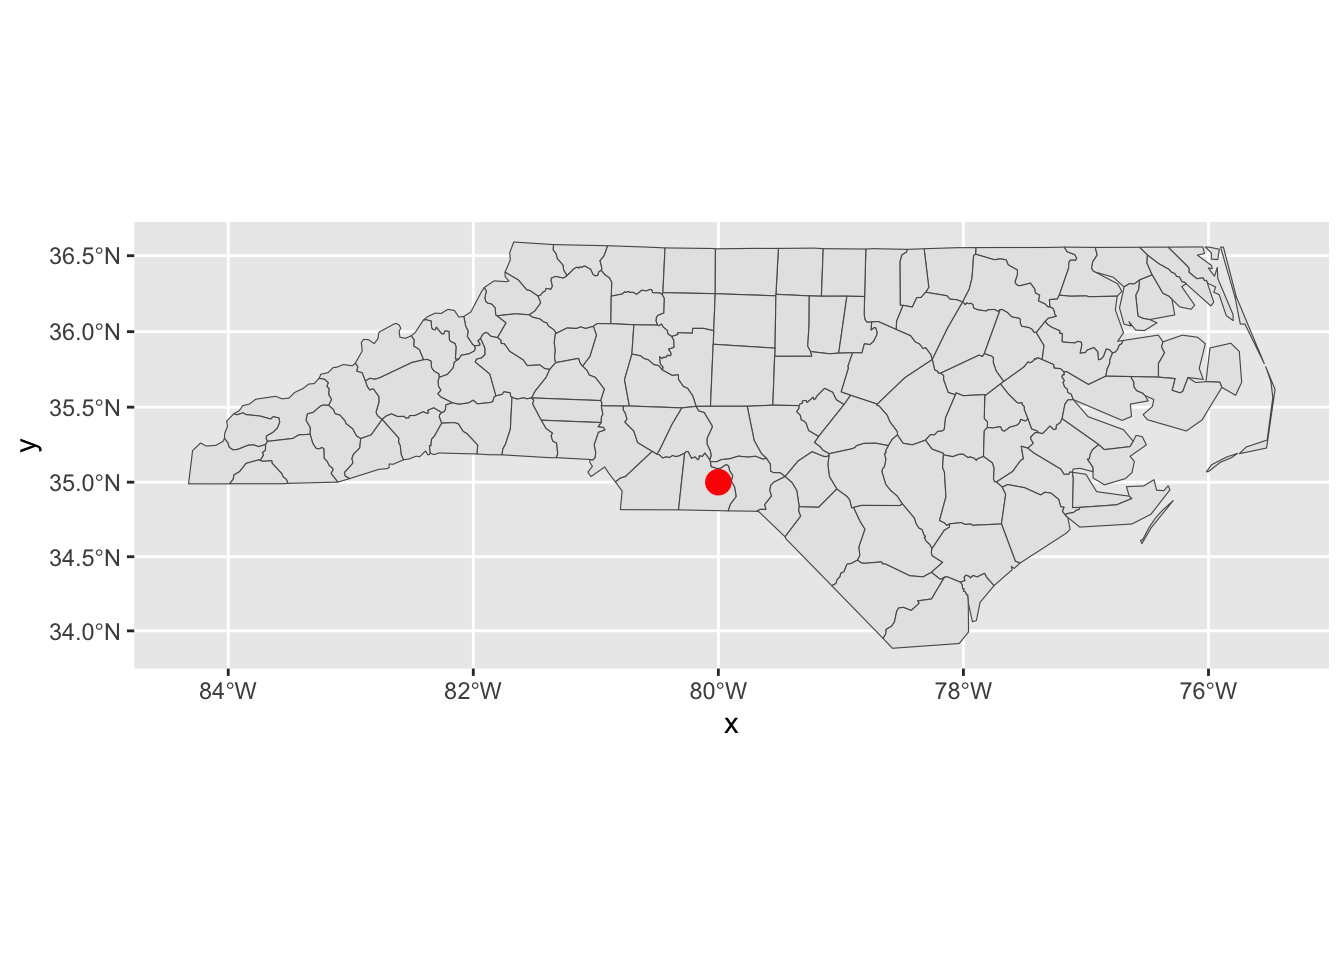
\includegraphics{eda1_files/figure-latex/unnamed-chunk-6-1.pdf}

\begin{center}\rule{0.5\linewidth}{0.5pt}\end{center}

\begin{Shaded}
\begin{Highlighting}[]
\FunctionTok{lm}\NormalTok{(cars}\SpecialCharTok{$}\NormalTok{dist}\SpecialCharTok{\textasciitilde{}}\NormalTok{cars}\SpecialCharTok{$}\NormalTok{speed)}
\end{Highlighting}
\end{Shaded}

\begin{verbatim}
## 
## Call:
## lm(formula = cars$dist ~ cars$speed)
## 
## Coefficients:
## (Intercept)   cars$speed  
##     -17.579        3.932
\end{verbatim}

\begin{center}\rule{0.5\linewidth}{0.5pt}\end{center}

\begin{Shaded}
\begin{Highlighting}[]
\FunctionTok{summary}\NormalTok{(}\FunctionTok{lm}\NormalTok{(cars}\SpecialCharTok{$}\NormalTok{dist}\SpecialCharTok{\textasciitilde{}}\NormalTok{cars}\SpecialCharTok{$}\NormalTok{speed))}
\end{Highlighting}
\end{Shaded}

\begin{verbatim}
## 
## Call:
## lm(formula = cars$dist ~ cars$speed)
## 
## Residuals:
##     Min      1Q  Median      3Q     Max 
## -29.069  -9.525  -2.272   9.215  43.201 
## 
## Coefficients:
##             Estimate Std. Error t value Pr(>|t|)    
## (Intercept) -17.5791     6.7584  -2.601   0.0123 *  
## cars$speed    3.9324     0.4155   9.464 1.49e-12 ***
## ---
## Signif. codes:  0 '***' 0.001 '**' 0.01 '*' 0.05 '.' 0.1 ' ' 1
## 
## Residual standard error: 15.38 on 48 degrees of freedom
## Multiple R-squared:  0.6511, Adjusted R-squared:  0.6438 
## F-statistic: 89.57 on 1 and 48 DF,  p-value: 1.49e-12
\end{verbatim}

\begin{center}\rule{0.5\linewidth}{0.5pt}\end{center}

\hypertarget{brief-explanation}{%
\paragraph{Brief Explanation}\label{brief-explanation}}

\begin{itemize}
\tightlist
\item
  \texttt{head(cars)}: The first 6 rows of the pre-installed data
  \texttt{cars}.
\item
  \texttt{str(cars)}: The data structure of the pre-installed data
  \texttt{cars}.
\item
  \texttt{summary(cars)}: The summary of the pre-installed data
  \texttt{cars}.
\item
  \texttt{plot(cars)}: A scatter plot of the pre-installed data
  \texttt{cars}.

  \begin{itemize}
  \tightlist
  \item
    \texttt{plot(cars\$dist\textasciitilde{}cars\$speed)}
  \item
    \texttt{cars\$dist}, \texttt{cars\${[}{[}2{]}{]}},
    \texttt{cars{[},2{]}} are same
  \end{itemize}
\item
  \texttt{abline(lm(cars\$dist\textasciitilde{}cars\$speed))}: Add a
  regression line of a linear model
\item
  \texttt{lm(cars\$dist\textasciitilde{}cars\$speed)}: The equation of
  the regression line
\item
  \texttt{summary(lm(cars\$dist\textasciitilde{}cars\$speed)}: The
  summary of the linear regression model
\end{itemize}

\begin{center}\rule{0.5\linewidth}{0.5pt}\end{center}

\begin{Shaded}
\begin{Highlighting}[]
\FunctionTok{hist}\NormalTok{(cars}\SpecialCharTok{$}\NormalTok{dist)}
\end{Highlighting}
\end{Shaded}

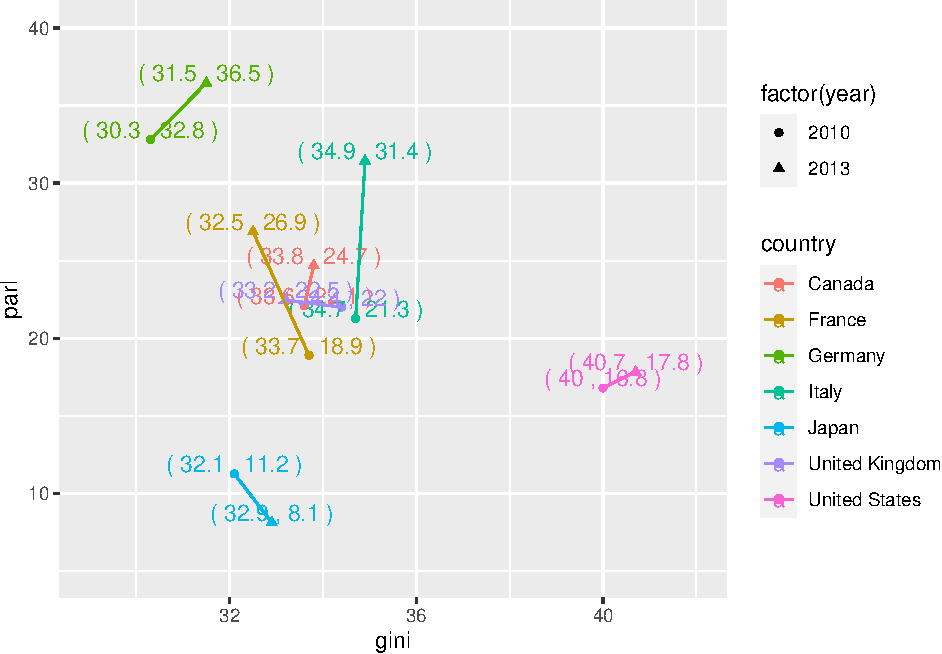
\includegraphics{eda1_files/figure-latex/unnamed-chunk-10-1.pdf}

\begin{center}\rule{0.5\linewidth}{0.5pt}\end{center}

\begin{Shaded}
\begin{Highlighting}[]
\FunctionTok{hist}\NormalTok{(cars}\SpecialCharTok{$}\NormalTok{speed)}
\end{Highlighting}
\end{Shaded}

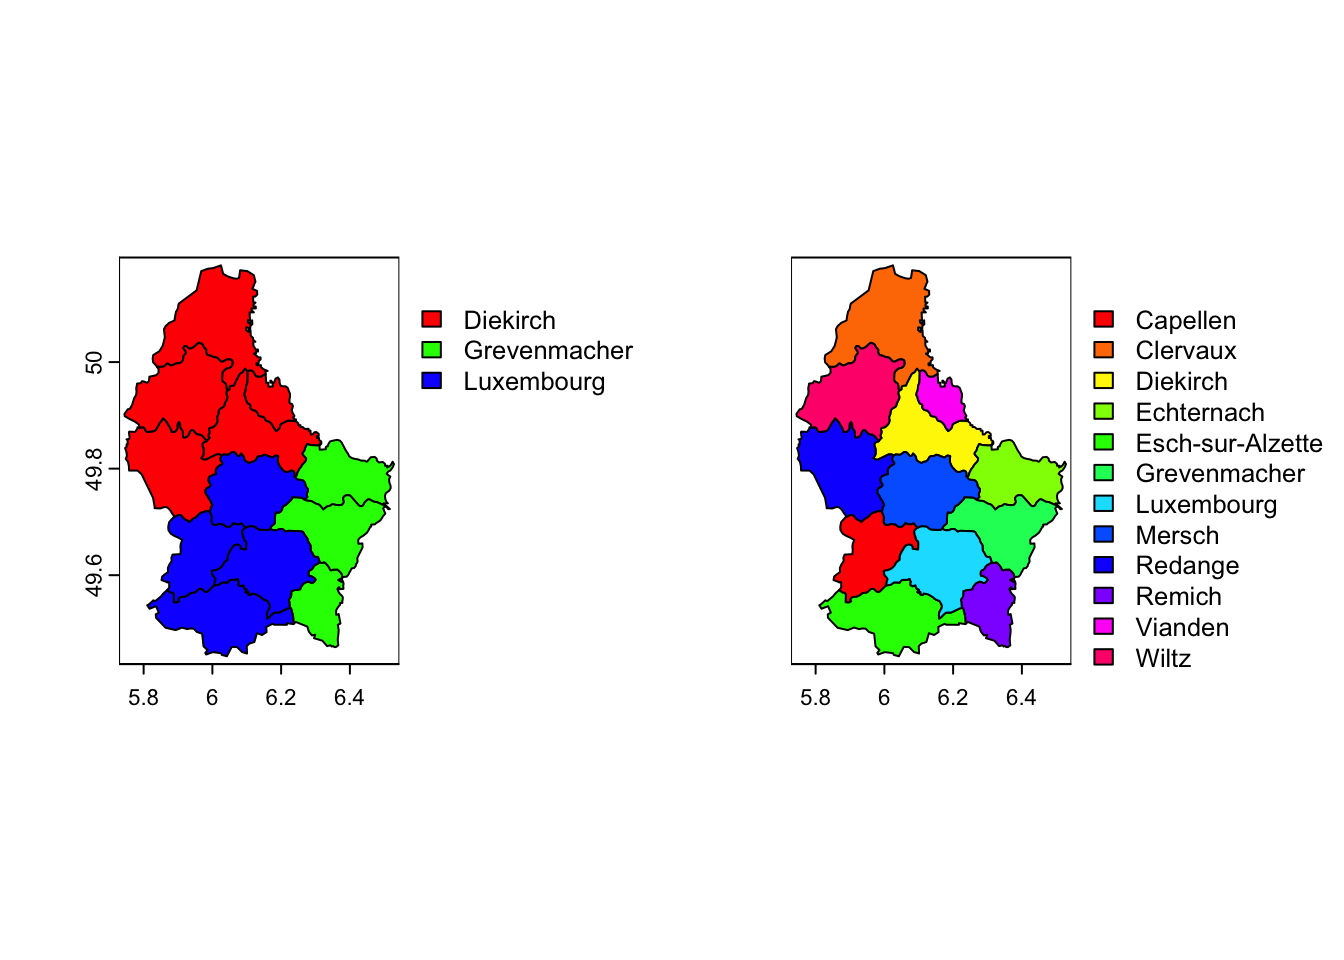
\includegraphics{eda1_files/figure-latex/unnamed-chunk-12-1.pdf}

\begin{center}\rule{0.5\linewidth}{0.5pt}\end{center}

\hypertarget{view-and-help}{%
\paragraph{View and help}\label{view-and-help}}

\begin{itemize}
\tightlist
\item
  \texttt{View(cars)}
\item
  \texttt{?cars}: same as \texttt{help(cars)}
\item
  \texttt{??cars}: same as `help.search(``cars'')
\end{itemize}

\hypertarget{datasets}{%
\paragraph{\texorpdfstring{\texttt{datasets}}{datasets}}\label{datasets}}

\begin{itemize}
\item
  \texttt{?datasets}
\item
  \texttt{library(help\ =\ "datasets")}
\item
  \texttt{data()} shows all data already attached and available.
\end{itemize}

\begin{center}\rule{0.5\linewidth}{0.5pt}\end{center}

\hypertarget{practicum}{%
\subsubsection{Practicum}\label{practicum}}

Pick a data in the datasets package and try

\begin{itemize}
\tightlist
\item
  \texttt{head()}
\item
  \texttt{str()}
\item
  \texttt{summary()}
\end{itemize}

and some more.

\begin{center}\rule{0.5\linewidth}{0.5pt}\end{center}

\hypertarget{iris}{%
\paragraph{\texorpdfstring{\texttt{iris}}{iris}}\label{iris}}

\begin{Shaded}
\begin{Highlighting}[]
\FunctionTok{head}\NormalTok{(iris)}
\end{Highlighting}
\end{Shaded}

\begin{verbatim}
##   Sepal.Length Sepal.Width Petal.Length Petal.Width Species
## 1          5.1         3.5          1.4         0.2  setosa
## 2          4.9         3.0          1.4         0.2  setosa
## 3          4.7         3.2          1.3         0.2  setosa
## 4          4.6         3.1          1.5         0.2  setosa
## 5          5.0         3.6          1.4         0.2  setosa
## 6          5.4         3.9          1.7         0.4  setosa
\end{verbatim}

\begin{center}\rule{0.5\linewidth}{0.5pt}\end{center}

\begin{Shaded}
\begin{Highlighting}[]
\FunctionTok{str}\NormalTok{(iris)}
\end{Highlighting}
\end{Shaded}

\begin{verbatim}
## 'data.frame':    150 obs. of  5 variables:
##  $ Sepal.Length: num  5.1 4.9 4.7 4.6 5 5.4 4.6 5 4.4 4.9 ...
##  $ Sepal.Width : num  3.5 3 3.2 3.1 3.6 3.9 3.4 3.4 2.9 3.1 ...
##  $ Petal.Length: num  1.4 1.4 1.3 1.5 1.4 1.7 1.4 1.5 1.4 1.5 ...
##  $ Petal.Width : num  0.2 0.2 0.2 0.2 0.2 0.4 0.3 0.2 0.2 0.1 ...
##  $ Species     : Factor w/ 3 levels "setosa","versicolor",..: 1 1 1 1 1 1 1 1 1 1 ...
\end{verbatim}

\begin{center}\rule{0.5\linewidth}{0.5pt}\end{center}

\begin{Shaded}
\begin{Highlighting}[]
\FunctionTok{summary}\NormalTok{(iris)}
\end{Highlighting}
\end{Shaded}

\begin{verbatim}
##   Sepal.Length    Sepal.Width     Petal.Length    Petal.Width   
##  Min.   :4.300   Min.   :2.000   Min.   :1.000   Min.   :0.100  
##  1st Qu.:5.100   1st Qu.:2.800   1st Qu.:1.600   1st Qu.:0.300  
##  Median :5.800   Median :3.000   Median :4.350   Median :1.300  
##  Mean   :5.843   Mean   :3.057   Mean   :3.758   Mean   :1.199  
##  3rd Qu.:6.400   3rd Qu.:3.300   3rd Qu.:5.100   3rd Qu.:1.800  
##  Max.   :7.900   Max.   :4.400   Max.   :6.900   Max.   :2.500  
##        Species  
##  setosa    :50  
##  versicolor:50  
##  virginica :50  
##                 
##                 
## 
\end{verbatim}

\begin{center}\rule{0.5\linewidth}{0.5pt}\end{center}

Can you plot?

\begin{Shaded}
\begin{Highlighting}[]
\FunctionTok{plot}\NormalTok{(iris}\SpecialCharTok{$}\NormalTok{Sepal.Length, iris}\SpecialCharTok{$}\NormalTok{Sepal.Width)}
\end{Highlighting}
\end{Shaded}

\includegraphics{eda1_files/figure-latex/unnamed-chunk-17-1.pdf}

\hypertarget{tidyverse-packages}{%
\subsection{\texorpdfstring{\texttt{tidyverse}
Packages}{tidyverse Packages}}\label{tidyverse-packages}}

\hypertarget{brief-introduction-to-r-on-rstudio}{%
\subsubsection{Brief Introduction to R on
RStudio}\label{brief-introduction-to-r-on-rstudio}}

\hypertarget{four-panes-and-tabs}{%
\paragraph{Four Panes and Tabs}\label{four-panes-and-tabs}}

\begin{enumerate}
\def\labelenumi{\arabic{enumi}.}
\tightlist
\item
  Top Left: Source Editor
\item
  Top Right: Environment, History, etc.
\item
  Bottom Left: Console, Terminal, Render, Background Jobs
\item
  Bottom Right: Files, Plots, Packages, Help, Viewer, Presentation
\end{enumerate}

\begin{center}\rule{0.5\linewidth}{0.5pt}\end{center}

\hypertarget{set-up}{%
\paragraph{Set up}\label{set-up}}

\begin{itemize}
\tightlist
\item
  Highly recommend to set the language to be ``English''.
\item
  Create ``data'' directory.
\end{itemize}

\begin{Shaded}
\begin{Highlighting}[]
\FunctionTok{Sys.setenv}\NormalTok{(}\AttributeTok{LANG =} \StringTok{"en"}\NormalTok{)}
\FunctionTok{dir.create}\NormalTok{(}\StringTok{"data"}\NormalTok{)}
\end{Highlighting}
\end{Shaded}

\begin{center}\rule{0.5\linewidth}{0.5pt}\end{center}

\hypertarget{three-ways-to-run-codes}{%
\paragraph{Three Ways to Run Codes}\label{three-ways-to-run-codes}}

\begin{enumerate}
\def\labelenumi{\arabic{enumi}.}
\tightlist
\item
  Console - Bottom Left Pane
\item
  R Script - pull down menu under File
\item
  R Notebook, R Markdown - pull down menu under File
\end{enumerate}

\begin{center}\rule{0.5\linewidth}{0.5pt}\end{center}

\hypertarget{second-way-r-script}{%
\subsubsection{Second Way: R Script}\label{second-way-r-script}}

\hypertarget{examples-r-scripts-in-moodle}{%
\paragraph{Examples: R Scripts in
Moodle}\label{examples-r-scripts-in-moodle}}

\begin{itemize}
\tightlist
\item
  \texttt{basics.R}
\item
  \texttt{coronavirus.R}
\end{itemize}

\begin{enumerate}
\def\labelenumi{\arabic{enumi}.}
\tightlist
\item
  Copy a script in Moodle: \emph{\{file name\}.R}
\item
  In RStudio (create Project in RStudio) choose File \textgreater{} New
  File \textgreater{} R Script and paste it.
\item
  Choose File \textgreater{} Save with a name; e.g.~\emph{\{file
  names\}} (.R will be added automatically)
\end{enumerate}

To run a code: at the cursor press \emph{Ctrl+Shift+Enter} (Win) or
\emph{Cmd+Shift+Enter} (Mac).

\begin{center}\rule{0.5\linewidth}{0.5pt}\end{center}

\hypertarget{packages}{%
\subsubsection{Packages}\label{packages}}

R packages are extensions to the R statistical programming language. R
packages contain code, data, and documentation in a standardised
collection format that can be installed by users of R, typically via a
centralised software repository such as CRAN (the Comprehensive R
Archive Network).

\hypertarget{installation-and-attachement}{%
\paragraph{Installation and
attachement}\label{installation-and-attachement}}

You can install packages by ``Install Packages\ldots{}'' under ``Tool''
in the top menu.

\begin{itemize}
\tightlist
\item
  \texttt{install.packages("tidyverse")}
\item
  \texttt{install.packages("rmarkdown")}
\end{itemize}

\begin{center}\rule{0.5\linewidth}{0.5pt}\end{center}

\hypertarget{third-way-r-notebook}{%
\subsubsection{Third Way: R Notebook}\label{third-way-r-notebook}}

Choose R Notebook from the pull down File menu in the top bar.

\hypertarget{edit-yaml}{%
\subsubsection{Edit YAML}\label{edit-yaml}}

\textbf{Default* is as follows}

\begin{verbatim}
---
title: "R Notebook"
output: html_notebook
---
\end{verbatim}

\begin{center}\rule{0.5\linewidth}{0.5pt}\end{center}

\textbf{Template}

\begin{verbatim}
---
title: "Title of R Notebook"
author: "ID and Your Name"
date: "2022-12-16" 
output: 
  html_notebook:
#    number_sections: yes
#    toc: true
#    toc_float: true
---
\end{verbatim}

\begin{itemize}
\tightlist
\item
  Don't change the format. Indention matters.
\item
  The statement after \# is ignored.
\item
  Date is automatically inserted when you compile the file.
\item
  You can replace ``2022-12-16'' by ``2022-12-14'' or in any date format
  surrounded by double quotation marks.
\item
  Section numbers: - default is \texttt{number\_sections:\ no}.
\item
  Table of contents, \texttt{toc:\ true} - default is
  \texttt{toc:\ false}.
\item
  Floating table of contents in HTML output, \texttt{toc\_float:\ true}
  - default is \texttt{toc\_float:\ false}
\end{itemize}

\begin{center}\rule{0.5\linewidth}{0.5pt}\end{center}

\hypertarget{create-a-code-chunk-to-attach-packages}{%
\subsubsection{Create a Code Chunk to Attach
Packages}\label{create-a-code-chunk-to-attach-packages}}

Insert Chunk in Code pull down menu in the top bar, or use the C button
on top. You can use shortcut keys listed under Tools in the top bar.

\begin{Shaded}
\begin{Highlighting}[]
\FunctionTok{library}\NormalTok{(tidyverse)}
\end{Highlighting}
\end{Shaded}

\begin{verbatim}
## -- Attaching packages --------------------------------------- tidyverse 1.3.2 --
## v ggplot2 3.4.0      v purrr   0.3.5 
## v tibble  3.1.8      v dplyr   1.0.10
## v tidyr   1.2.1      v stringr 1.4.1 
## v readr   2.1.3      v forcats 0.5.2 
## -- Conflicts ------------------------------------------ tidyverse_conflicts() --
## x dplyr::filter() masks stats::filter()
## x dplyr::lag()    masks stats::lag()
\end{verbatim}

\hypertarget{first-example}{%
\subsection{First Example}\label{first-example}}

\hypertarget{importing-data}{%
\subsubsection{Importing data}\label{importing-data}}

Let us assign the \texttt{iris} data in the pre-installed package
\texttt{datasets} to \texttt{df\_iris}. You can give any name starting
from an alphabet, though there are some rules.

\begin{Shaded}
\begin{Highlighting}[]
\NormalTok{df\_iris }\OtherTok{\textless{}{-}}\NormalTok{ datasets}\SpecialCharTok{::}\NormalTok{iris}
\FunctionTok{class}\NormalTok{(df\_iris)}
\end{Highlighting}
\end{Shaded}

\begin{verbatim}
## [1] "data.frame"
\end{verbatim}

The class of data \texttt{iris} is \texttt{data.frame}, the basic data
class of R. You can assign the same data as a \texttt{tibble}, the data
class of \texttt{tidyverse} as follows.

\begin{Shaded}
\begin{Highlighting}[]
\NormalTok{tbl\_iris }\OtherTok{\textless{}{-}} \FunctionTok{as\_tibble}\NormalTok{(datasets}\SpecialCharTok{::}\NormalTok{iris)}
\FunctionTok{class}\NormalTok{(tbl\_iris)}
\end{Highlighting}
\end{Shaded}

\begin{verbatim}
## [1] "tbl_df"     "tbl"        "data.frame"
\end{verbatim}

\begin{itemize}
\tightlist
\item
  \texttt{df\_iris\ \textless{}-\ iris} can replace
  \texttt{df\_iris\ \textless{}-\ datasets::iris} because the package
  \texttt{datasets} is installed and attached as default. Since you may
  have other data called \texttt{iris} included in a different package
  or you may have changed \texttt{iris} before, it is safer to specify
  the name of the package with the name of the data.
\item
  Within R Notebook or in Console, you may get different output, and
  \texttt{tf\_iris} and \texttt{tbl\_iris} behave differently. It is
  because of the default settings of R Markdown.
\end{itemize}

\begin{center}\rule{0.5\linewidth}{0.5pt}\end{center}

\hypertarget{look-at-the-data}{%
\subsubsection{Look at the data}\label{look-at-the-data}}

\hypertarget{several-ways-to-view-the-data.}{%
\paragraph{Several ways to view the
data.}\label{several-ways-to-view-the-data.}}

The \texttt{View} command open up a window to show the contents of the
data and you can use the filter as well.

\begin{Shaded}
\begin{Highlighting}[]
\FunctionTok{View}\NormalTok{(df\_iris)}
\end{Highlighting}
\end{Shaded}

\begin{center}\rule{0.5\linewidth}{0.5pt}\end{center}

The following simple command also shows the data.

\begin{Shaded}
\begin{Highlighting}[]
\NormalTok{df\_iris}
\end{Highlighting}
\end{Shaded}

\begin{verbatim}
##     Sepal.Length Sepal.Width Petal.Length Petal.Width    Species
## 1            5.1         3.5          1.4         0.2     setosa
## 2            4.9         3.0          1.4         0.2     setosa
## 3            4.7         3.2          1.3         0.2     setosa
## 4            4.6         3.1          1.5         0.2     setosa
## 5            5.0         3.6          1.4         0.2     setosa
## 6            5.4         3.9          1.7         0.4     setosa
## 7            4.6         3.4          1.4         0.3     setosa
## 8            5.0         3.4          1.5         0.2     setosa
## 9            4.4         2.9          1.4         0.2     setosa
## 10           4.9         3.1          1.5         0.1     setosa
## 11           5.4         3.7          1.5         0.2     setosa
## 12           4.8         3.4          1.6         0.2     setosa
## 13           4.8         3.0          1.4         0.1     setosa
## 14           4.3         3.0          1.1         0.1     setosa
## 15           5.8         4.0          1.2         0.2     setosa
## 16           5.7         4.4          1.5         0.4     setosa
## 17           5.4         3.9          1.3         0.4     setosa
## 18           5.1         3.5          1.4         0.3     setosa
## 19           5.7         3.8          1.7         0.3     setosa
## 20           5.1         3.8          1.5         0.3     setosa
## 21           5.4         3.4          1.7         0.2     setosa
## 22           5.1         3.7          1.5         0.4     setosa
## 23           4.6         3.6          1.0         0.2     setosa
## 24           5.1         3.3          1.7         0.5     setosa
## 25           4.8         3.4          1.9         0.2     setosa
## 26           5.0         3.0          1.6         0.2     setosa
## 27           5.0         3.4          1.6         0.4     setosa
## 28           5.2         3.5          1.5         0.2     setosa
## 29           5.2         3.4          1.4         0.2     setosa
## 30           4.7         3.2          1.6         0.2     setosa
## 31           4.8         3.1          1.6         0.2     setosa
## 32           5.4         3.4          1.5         0.4     setosa
## 33           5.2         4.1          1.5         0.1     setosa
## 34           5.5         4.2          1.4         0.2     setosa
## 35           4.9         3.1          1.5         0.2     setosa
## 36           5.0         3.2          1.2         0.2     setosa
## 37           5.5         3.5          1.3         0.2     setosa
## 38           4.9         3.6          1.4         0.1     setosa
## 39           4.4         3.0          1.3         0.2     setosa
## 40           5.1         3.4          1.5         0.2     setosa
## 41           5.0         3.5          1.3         0.3     setosa
## 42           4.5         2.3          1.3         0.3     setosa
## 43           4.4         3.2          1.3         0.2     setosa
## 44           5.0         3.5          1.6         0.6     setosa
## 45           5.1         3.8          1.9         0.4     setosa
## 46           4.8         3.0          1.4         0.3     setosa
## 47           5.1         3.8          1.6         0.2     setosa
## 48           4.6         3.2          1.4         0.2     setosa
## 49           5.3         3.7          1.5         0.2     setosa
## 50           5.0         3.3          1.4         0.2     setosa
## 51           7.0         3.2          4.7         1.4 versicolor
## 52           6.4         3.2          4.5         1.5 versicolor
## 53           6.9         3.1          4.9         1.5 versicolor
## 54           5.5         2.3          4.0         1.3 versicolor
## 55           6.5         2.8          4.6         1.5 versicolor
## 56           5.7         2.8          4.5         1.3 versicolor
## 57           6.3         3.3          4.7         1.6 versicolor
## 58           4.9         2.4          3.3         1.0 versicolor
## 59           6.6         2.9          4.6         1.3 versicolor
## 60           5.2         2.7          3.9         1.4 versicolor
## 61           5.0         2.0          3.5         1.0 versicolor
## 62           5.9         3.0          4.2         1.5 versicolor
## 63           6.0         2.2          4.0         1.0 versicolor
## 64           6.1         2.9          4.7         1.4 versicolor
## 65           5.6         2.9          3.6         1.3 versicolor
## 66           6.7         3.1          4.4         1.4 versicolor
## 67           5.6         3.0          4.5         1.5 versicolor
## 68           5.8         2.7          4.1         1.0 versicolor
## 69           6.2         2.2          4.5         1.5 versicolor
## 70           5.6         2.5          3.9         1.1 versicolor
## 71           5.9         3.2          4.8         1.8 versicolor
## 72           6.1         2.8          4.0         1.3 versicolor
## 73           6.3         2.5          4.9         1.5 versicolor
## 74           6.1         2.8          4.7         1.2 versicolor
## 75           6.4         2.9          4.3         1.3 versicolor
## 76           6.6         3.0          4.4         1.4 versicolor
## 77           6.8         2.8          4.8         1.4 versicolor
## 78           6.7         3.0          5.0         1.7 versicolor
## 79           6.0         2.9          4.5         1.5 versicolor
## 80           5.7         2.6          3.5         1.0 versicolor
## 81           5.5         2.4          3.8         1.1 versicolor
## 82           5.5         2.4          3.7         1.0 versicolor
## 83           5.8         2.7          3.9         1.2 versicolor
## 84           6.0         2.7          5.1         1.6 versicolor
## 85           5.4         3.0          4.5         1.5 versicolor
## 86           6.0         3.4          4.5         1.6 versicolor
## 87           6.7         3.1          4.7         1.5 versicolor
## 88           6.3         2.3          4.4         1.3 versicolor
## 89           5.6         3.0          4.1         1.3 versicolor
## 90           5.5         2.5          4.0         1.3 versicolor
## 91           5.5         2.6          4.4         1.2 versicolor
## 92           6.1         3.0          4.6         1.4 versicolor
## 93           5.8         2.6          4.0         1.2 versicolor
## 94           5.0         2.3          3.3         1.0 versicolor
## 95           5.6         2.7          4.2         1.3 versicolor
## 96           5.7         3.0          4.2         1.2 versicolor
## 97           5.7         2.9          4.2         1.3 versicolor
## 98           6.2         2.9          4.3         1.3 versicolor
## 99           5.1         2.5          3.0         1.1 versicolor
## 100          5.7         2.8          4.1         1.3 versicolor
## 101          6.3         3.3          6.0         2.5  virginica
## 102          5.8         2.7          5.1         1.9  virginica
## 103          7.1         3.0          5.9         2.1  virginica
## 104          6.3         2.9          5.6         1.8  virginica
## 105          6.5         3.0          5.8         2.2  virginica
## 106          7.6         3.0          6.6         2.1  virginica
## 107          4.9         2.5          4.5         1.7  virginica
## 108          7.3         2.9          6.3         1.8  virginica
## 109          6.7         2.5          5.8         1.8  virginica
## 110          7.2         3.6          6.1         2.5  virginica
## 111          6.5         3.2          5.1         2.0  virginica
## 112          6.4         2.7          5.3         1.9  virginica
## 113          6.8         3.0          5.5         2.1  virginica
## 114          5.7         2.5          5.0         2.0  virginica
## 115          5.8         2.8          5.1         2.4  virginica
## 116          6.4         3.2          5.3         2.3  virginica
## 117          6.5         3.0          5.5         1.8  virginica
## 118          7.7         3.8          6.7         2.2  virginica
## 119          7.7         2.6          6.9         2.3  virginica
## 120          6.0         2.2          5.0         1.5  virginica
## 121          6.9         3.2          5.7         2.3  virginica
## 122          5.6         2.8          4.9         2.0  virginica
## 123          7.7         2.8          6.7         2.0  virginica
## 124          6.3         2.7          4.9         1.8  virginica
## 125          6.7         3.3          5.7         2.1  virginica
## 126          7.2         3.2          6.0         1.8  virginica
## 127          6.2         2.8          4.8         1.8  virginica
## 128          6.1         3.0          4.9         1.8  virginica
## 129          6.4         2.8          5.6         2.1  virginica
## 130          7.2         3.0          5.8         1.6  virginica
## 131          7.4         2.8          6.1         1.9  virginica
## 132          7.9         3.8          6.4         2.0  virginica
## 133          6.4         2.8          5.6         2.2  virginica
## 134          6.3         2.8          5.1         1.5  virginica
## 135          6.1         2.6          5.6         1.4  virginica
## 136          7.7         3.0          6.1         2.3  virginica
## 137          6.3         3.4          5.6         2.4  virginica
## 138          6.4         3.1          5.5         1.8  virginica
## 139          6.0         3.0          4.8         1.8  virginica
## 140          6.9         3.1          5.4         2.1  virginica
## 141          6.7         3.1          5.6         2.4  virginica
## 142          6.9         3.1          5.1         2.3  virginica
## 143          5.8         2.7          5.1         1.9  virginica
## 144          6.8         3.2          5.9         2.3  virginica
## 145          6.7         3.3          5.7         2.5  virginica
## 146          6.7         3.0          5.2         2.3  virginica
## 147          6.3         2.5          5.0         1.9  virginica
## 148          6.5         3.0          5.2         2.0  virginica
## 149          6.2         3.4          5.4         2.3  virginica
## 150          5.9         3.0          5.1         1.8  virginica
\end{verbatim}

The output within R Notebook is a tibble style. Try the same command in
Console.

\begin{center}\rule{0.5\linewidth}{0.5pt}\end{center}

\begin{Shaded}
\begin{Highlighting}[]
\FunctionTok{slice}\NormalTok{(df\_iris, }\DecValTok{1}\SpecialCharTok{:}\DecValTok{10}\NormalTok{)}
\end{Highlighting}
\end{Shaded}

\begin{verbatim}
##    Sepal.Length Sepal.Width Petal.Length Petal.Width Species
## 1           5.1         3.5          1.4         0.2  setosa
## 2           4.9         3.0          1.4         0.2  setosa
## 3           4.7         3.2          1.3         0.2  setosa
## 4           4.6         3.1          1.5         0.2  setosa
## 5           5.0         3.6          1.4         0.2  setosa
## 6           5.4         3.9          1.7         0.4  setosa
## 7           4.6         3.4          1.4         0.3  setosa
## 8           5.0         3.4          1.5         0.2  setosa
## 9           4.4         2.9          1.4         0.2  setosa
## 10          4.9         3.1          1.5         0.1  setosa
\end{verbatim}

\begin{Shaded}
\begin{Highlighting}[]
\DecValTok{1}\SpecialCharTok{:}\DecValTok{10}
\end{Highlighting}
\end{Shaded}

\begin{verbatim}
##  [1]  1  2  3  4  5  6  7  8  9 10
\end{verbatim}

\hypertarget{section}{%
\subsection{`}\label{section}}

\hypertarget{data-structure}{%
\paragraph{Data Structure}\label{data-structure}}

Let us look at the structure of the data. You can try
\texttt{str(df\_iris)} on Console or by adding a code chunk in R
Notebook introducing later.

\begin{Shaded}
\begin{Highlighting}[]
\FunctionTok{glimpse}\NormalTok{(df\_iris)}
\end{Highlighting}
\end{Shaded}

\begin{verbatim}
## Rows: 150
## Columns: 5
## $ Sepal.Length <dbl> 5.1, 4.9, 4.7, 4.6, 5.0, 5.4, 4.6, 5.0, 4.4, 4.9, 5.4, 4.~
## $ Sepal.Width  <dbl> 3.5, 3.0, 3.2, 3.1, 3.6, 3.9, 3.4, 3.4, 2.9, 3.1, 3.7, 3.~
## $ Petal.Length <dbl> 1.4, 1.4, 1.3, 1.5, 1.4, 1.7, 1.4, 1.5, 1.4, 1.5, 1.5, 1.~
## $ Petal.Width  <dbl> 0.2, 0.2, 0.2, 0.2, 0.2, 0.4, 0.3, 0.2, 0.2, 0.1, 0.2, 0.~
## $ Species      <fct> setosa, setosa, setosa, setosa, setosa, setosa, setosa, s~
\end{verbatim}

There are six types of data in R; Double, Integer, Character, Logical,
Raw, Complex.

The names after \$ are column names. If you call
\texttt{df\_iris\$Species}, you have the Species column. Species is in
the 5th collumn, \texttt{typeof(df\_iris{[}{[}5{]}{]})} does the same as
the next.

\texttt{df\_iris{[}2,4{]}\ =}0.2 is the fourth entry of Sepal.Width.

\begin{center}\rule{0.5\linewidth}{0.5pt}\end{center}

\begin{Shaded}
\begin{Highlighting}[]
\FunctionTok{typeof}\NormalTok{(df\_iris}\SpecialCharTok{$}\NormalTok{Species)}
\end{Highlighting}
\end{Shaded}

\begin{verbatim}
## [1] "integer"
\end{verbatim}

\begin{Shaded}
\begin{Highlighting}[]
\FunctionTok{class}\NormalTok{(df\_iris}\SpecialCharTok{$}\NormalTok{Species)}
\end{Highlighting}
\end{Shaded}

\begin{verbatim}
## [1] "factor"
\end{verbatim}

For \texttt{factors\ =\ fct} see
\href{https://www.rdocumentation.org/packages/base/versions/3.6.2/topics/factor}{the
R Document} or an explanation in
\href{https://www.guru99.com/r-factor-categorical-continuous.html}{Factor
in R: Categorical Variable \& Continuous Variables}.

\begin{center}\rule{0.5\linewidth}{0.5pt}\end{center}

\begin{Shaded}
\begin{Highlighting}[]
\FunctionTok{typeof}\NormalTok{(df\_iris}\SpecialCharTok{$}\NormalTok{Sepal.Length)}
\end{Highlighting}
\end{Shaded}

\begin{verbatim}
## [1] "double"
\end{verbatim}

\begin{Shaded}
\begin{Highlighting}[]
\FunctionTok{class}\NormalTok{(df\_iris}\SpecialCharTok{$}\NormalTok{Sepal.Length)}
\end{Highlighting}
\end{Shaded}

\begin{verbatim}
## [1] "numeric"
\end{verbatim}

\textbf{Q1.} What are the differences of\texttt{df\_iris},
\texttt{slice(df\_iris,\ 1:10)} and \texttt{glimpse(df\_iris)} above?

\textbf{Q2.} What are the differences of\texttt{df\_iris},
\texttt{slice(df\_iris,\ 1:10)} and \texttt{glimpse(df\_iris)} in the
console?

\begin{center}\rule{0.5\linewidth}{0.5pt}\end{center}

\hypertarget{summary-of-the-data}{%
\paragraph{Summary of the Data}\label{summary-of-the-data}}

The following is very convenient to get the summary information of a
data.

\begin{Shaded}
\begin{Highlighting}[]
\FunctionTok{summary}\NormalTok{(df\_iris)}
\end{Highlighting}
\end{Shaded}

\begin{verbatim}
##   Sepal.Length    Sepal.Width     Petal.Length    Petal.Width   
##  Min.   :4.300   Min.   :2.000   Min.   :1.000   Min.   :0.100  
##  1st Qu.:5.100   1st Qu.:2.800   1st Qu.:1.600   1st Qu.:0.300  
##  Median :5.800   Median :3.000   Median :4.350   Median :1.300  
##  Mean   :5.843   Mean   :3.057   Mean   :3.758   Mean   :1.199  
##  3rd Qu.:6.400   3rd Qu.:3.300   3rd Qu.:5.100   3rd Qu.:1.800  
##  Max.   :7.900   Max.   :4.400   Max.   :6.900   Max.   :2.500  
##        Species  
##  setosa    :50  
##  versicolor:50  
##  virginica :50  
##                 
##                 
## 
\end{verbatim}

Minimum, 1st Quadrant (25\%), Median, Mean, 3rd Quadrant (75\%),
Maximum, and the count of each factor.

\begin{center}\rule{0.5\linewidth}{0.5pt}\end{center}

\hypertarget{visualizing-data}{%
\subsubsection{Visualizing Data}\label{visualizing-data}}

\hypertarget{scatter-plot}{%
\paragraph{Scatter Plot}\label{scatter-plot}}

We use \texttt{ggplot} to draw graphs. The scatter plot is a projection
of data with two variables \(x\) and \(y\).

\begin{verbatim}
ggplot(data = <data>, aes(x = <column name for x>, y = <column name for y>)) +
  geom_point()
\end{verbatim}

\begin{verbatim}
ggplot(data = df_iris, aes(x = Sepal.Length, y = Sepal.Width)) +
  geom_point()
\end{verbatim}

\begin{center}\rule{0.5\linewidth}{0.5pt}\end{center}

\begin{Shaded}
\begin{Highlighting}[]
\FunctionTok{ggplot}\NormalTok{(}\AttributeTok{data =}\NormalTok{ df\_iris, }\FunctionTok{aes}\NormalTok{(}\AttributeTok{x =}\NormalTok{ Sepal.Length, }\AttributeTok{y =}\NormalTok{ Sepal.Width)) }\SpecialCharTok{+}
  \FunctionTok{geom\_point}\NormalTok{()}
\end{Highlighting}
\end{Shaded}

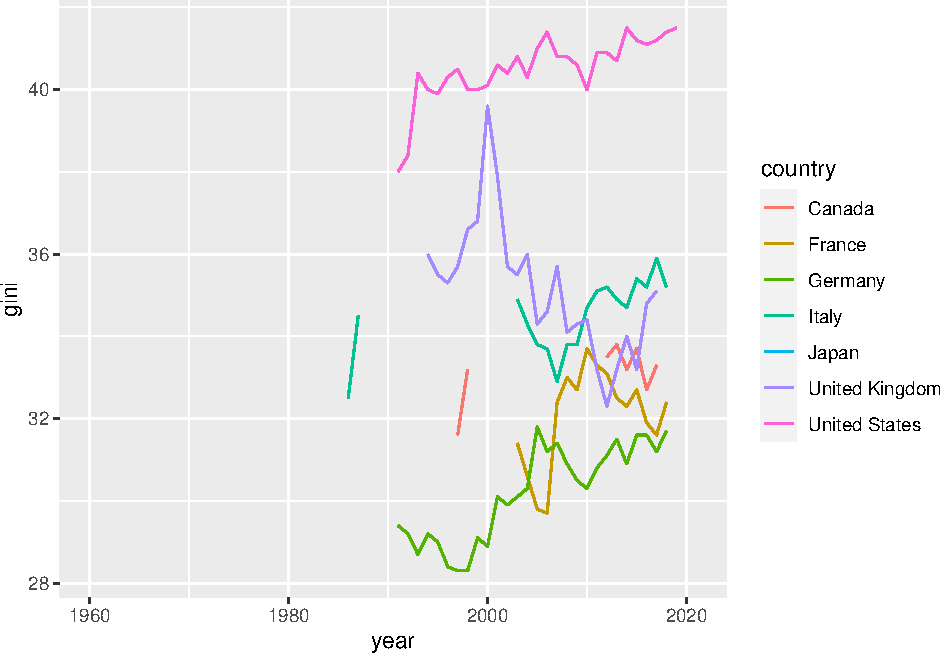
\includegraphics{eda1_files/figure-latex/unnamed-chunk-26-1.pdf}

\begin{center}\rule{0.5\linewidth}{0.5pt}\end{center}

\hypertarget{scatter-plot-with-labels}{%
\paragraph{\texorpdfstring{Scatter Plot with
\href{https://ggplot2.tidyverse.org/reference/labs.html}{Labels}}{Scatter Plot with Labels}}\label{scatter-plot-with-labels}}

Add title and labels adding \texttt{labs()}.

\begin{verbatim}
ggplot(data = <data>, aes(x = <column name for x>, y = <column name for y>)) +
  geom_point() +
  labs(title = "Title", x = "Label for x", y = "Label for y")
\end{verbatim}

\begin{center}\rule{0.5\linewidth}{0.5pt}\end{center}

\begin{Shaded}
\begin{Highlighting}[]
\FunctionTok{ggplot}\NormalTok{(}\AttributeTok{data =}\NormalTok{ df\_iris, }\FunctionTok{aes}\NormalTok{(}\AttributeTok{x =}\NormalTok{ Sepal.Length, }\AttributeTok{y =}\NormalTok{ Sepal.Width)) }\SpecialCharTok{+}
  \FunctionTok{geom\_point}\NormalTok{() }\SpecialCharTok{+} 
  \FunctionTok{labs}\NormalTok{(}\AttributeTok{title =} \StringTok{"Scatter Plot of Sepal Data of Iris"}\NormalTok{, }\AttributeTok{x =} \StringTok{"Sepal Length"}\NormalTok{, }\AttributeTok{y =} \StringTok{"Sepal Width"}\NormalTok{)}
\end{Highlighting}
\end{Shaded}

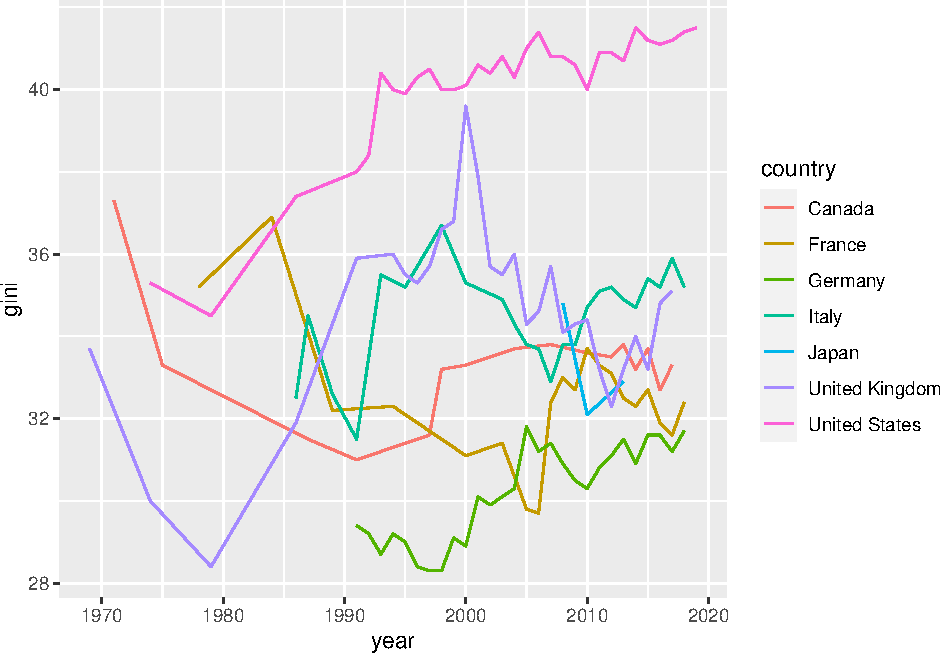
\includegraphics{eda1_files/figure-latex/unnamed-chunk-27-1.pdf}

\begin{center}\rule{0.5\linewidth}{0.5pt}\end{center}

\hypertarget{scatter-plot-with-colors}{%
\paragraph{\texorpdfstring{Scatter Plot with
\href{https://ggplot2.tidyverse.org/reference/aes_colour_fill_alpha.html}{Colors}}{Scatter Plot with Colors}}\label{scatter-plot-with-colors}}

Add different colors automatically to each species. Can you see each
group?

\begin{Shaded}
\begin{Highlighting}[]
\FunctionTok{ggplot}\NormalTok{(}\AttributeTok{data =}\NormalTok{ df\_iris, }\FunctionTok{aes}\NormalTok{(}\AttributeTok{x =}\NormalTok{ Sepal.Length, }\AttributeTok{y =}\NormalTok{ Sepal.Width, }\AttributeTok{color =}\NormalTok{ Species)) }\SpecialCharTok{+}
  \FunctionTok{geom\_point}\NormalTok{()}
\end{Highlighting}
\end{Shaded}

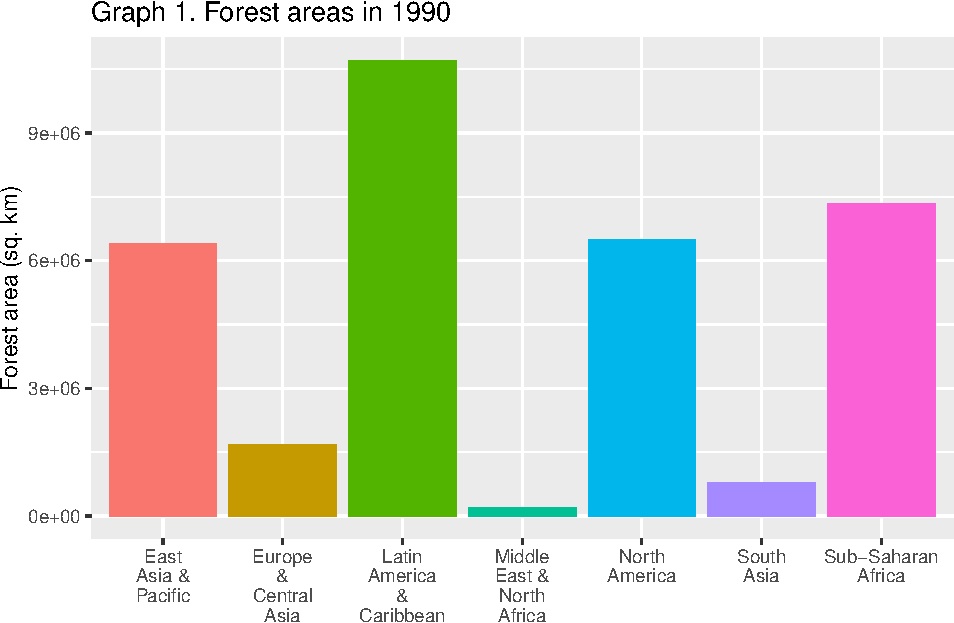
\includegraphics{eda1_files/figure-latex/unnamed-chunk-28-1.pdf}

\begin{center}\rule{0.5\linewidth}{0.5pt}\end{center}

\hypertarget{scatter-plot-with-shapes}{%
\paragraph{Scatter Plot with Shapes}\label{scatter-plot-with-shapes}}

\begin{Shaded}
\begin{Highlighting}[]
\FunctionTok{ggplot}\NormalTok{(}\AttributeTok{data =}\NormalTok{ df\_iris, }\FunctionTok{aes}\NormalTok{(}\AttributeTok{x =}\NormalTok{ Sepal.Length, }\AttributeTok{y =}\NormalTok{ Sepal.Width, }\AttributeTok{shape =}\NormalTok{ Species)) }\SpecialCharTok{+}
  \FunctionTok{geom\_point}\NormalTok{()}
\end{Highlighting}
\end{Shaded}

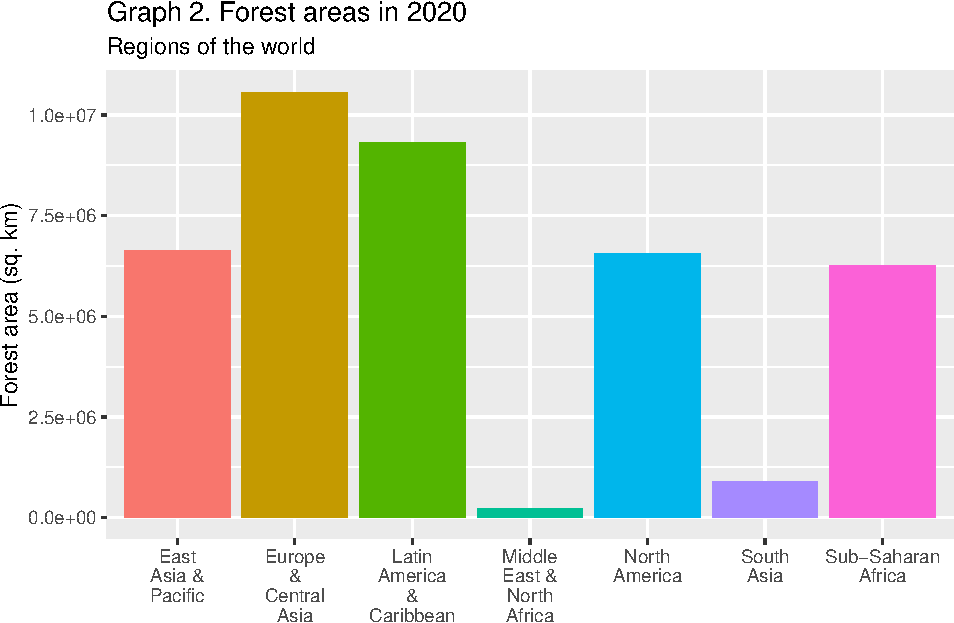
\includegraphics{eda1_files/figure-latex/unnamed-chunk-29-1.pdf}

\begin{center}\rule{0.5\linewidth}{0.5pt}\end{center}

\hypertarget{boxplot}{%
\paragraph{\texorpdfstring{\href{https://ggplot2.tidyverse.org/reference/geom_boxplot.html}{Boxplot}}{Boxplot}}\label{boxplot}}

The boxplot compactly displays the distribution of a continuous
variable.

\begin{Shaded}
\begin{Highlighting}[]
\FunctionTok{ggplot}\NormalTok{(}\AttributeTok{data =}\NormalTok{ df\_iris, }\FunctionTok{aes}\NormalTok{(}\AttributeTok{x =}\NormalTok{ Species, }\AttributeTok{y =}\NormalTok{ Sepal.Length)) }\SpecialCharTok{+}
  \FunctionTok{geom\_boxplot}\NormalTok{()}
\end{Highlighting}
\end{Shaded}

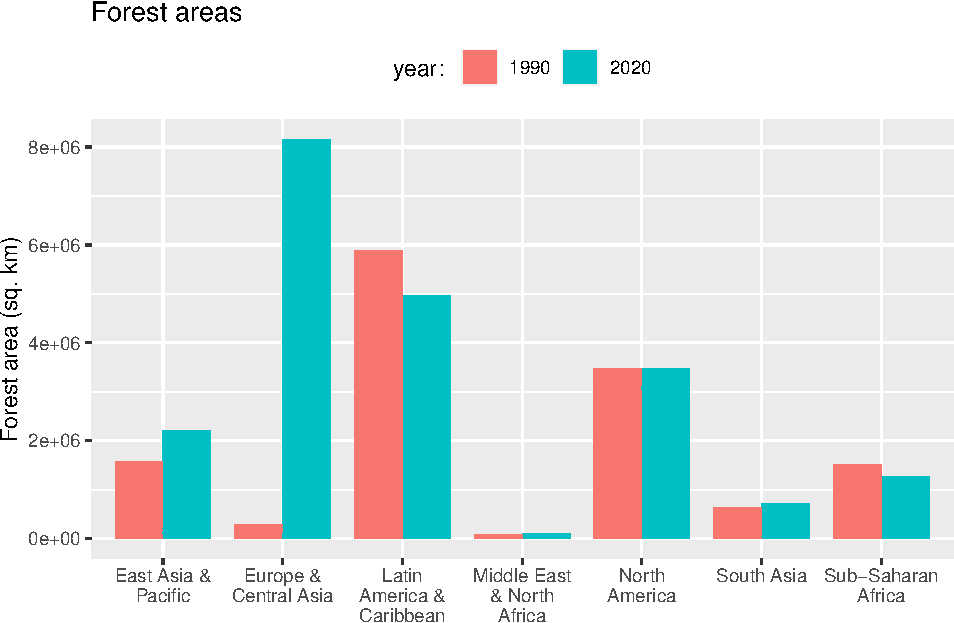
\includegraphics{eda1_files/figure-latex/unnamed-chunk-30-1.pdf}

\begin{center}\rule{0.5\linewidth}{0.5pt}\end{center}

\hypertarget{histogram}{%
\paragraph{\texorpdfstring{\href{https://ggplot2.tidyverse.org/reference/geom_histogram.html}{Histogram}}{Histogram}}\label{histogram}}

Visualize the distribution of a single continuous variable by dividing
the x axis into bins and counting the number of observations in each
bin. Histograms (geom\_histogram()) display the counts with bars.

\begin{Shaded}
\begin{Highlighting}[]
\FunctionTok{ggplot}\NormalTok{(}\AttributeTok{data =}\NormalTok{ df\_iris, }\FunctionTok{aes}\NormalTok{(}\AttributeTok{x =}\NormalTok{ Sepal.Length)) }\SpecialCharTok{+}
  \FunctionTok{geom\_histogram}\NormalTok{()}
\end{Highlighting}
\end{Shaded}

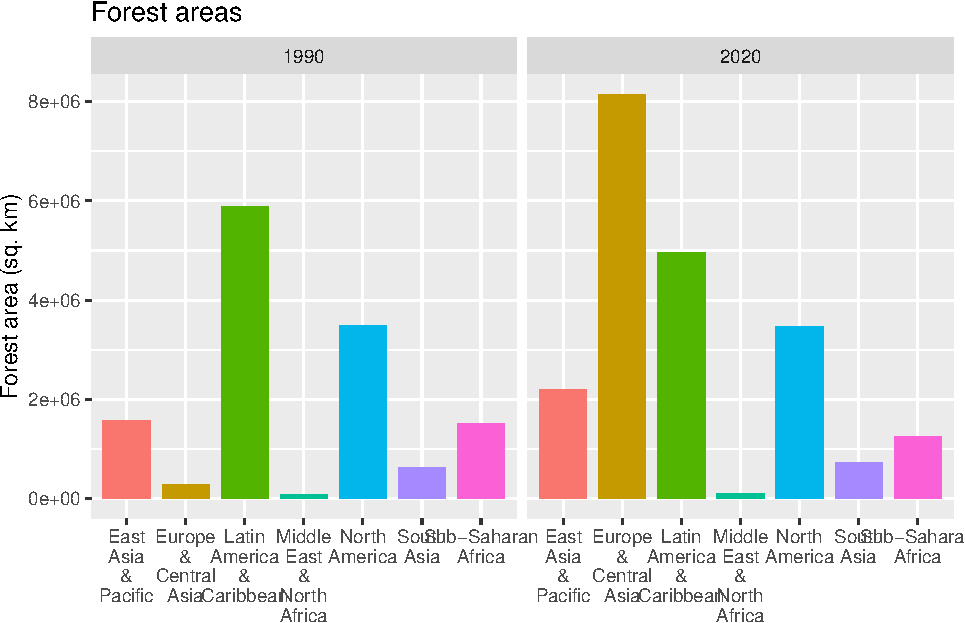
\includegraphics{eda1_files/figure-latex/unnamed-chunk-31-1.pdf}

\begin{center}\rule{0.5\linewidth}{0.5pt}\end{center}

Change the number of bins by \texttt{bins\ =}
\texttt{\textless{}number\textgreater{}}.

\begin{Shaded}
\begin{Highlighting}[]
\FunctionTok{ggplot}\NormalTok{(}\AttributeTok{data =}\NormalTok{ df\_iris, }\FunctionTok{aes}\NormalTok{(}\AttributeTok{x =}\NormalTok{ Sepal.Length)) }\SpecialCharTok{+}
  \FunctionTok{geom\_histogram}\NormalTok{(}\AttributeTok{bins =} \DecValTok{10}\NormalTok{)}
\end{Highlighting}
\end{Shaded}

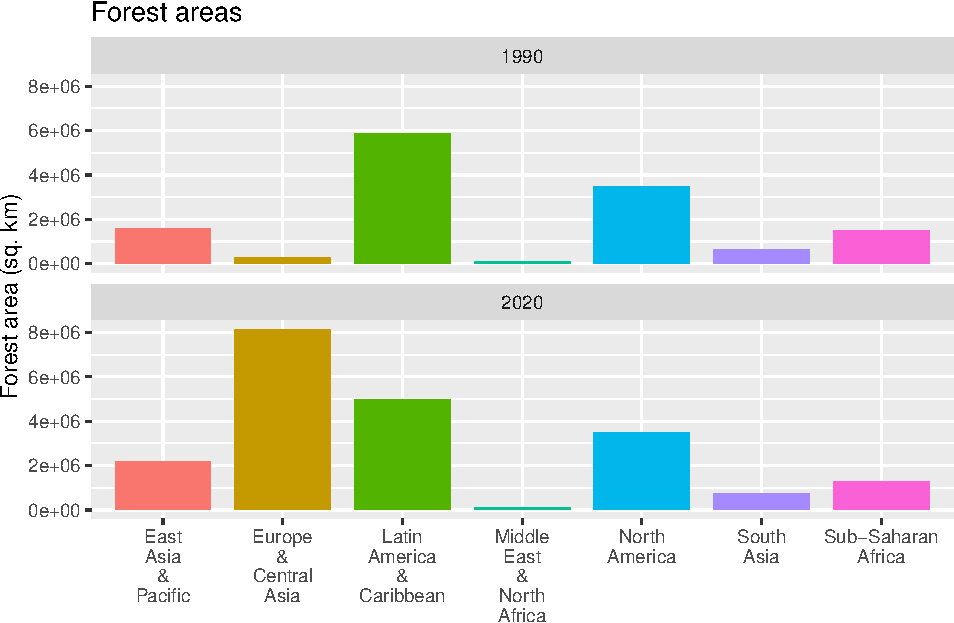
\includegraphics{eda1_files/figure-latex/unnamed-chunk-32-1.pdf}

\begin{center}\rule{0.5\linewidth}{0.5pt}\end{center}

\hypertarget{data-modeling}{%
\subsubsection{Data Modeling}\label{data-modeling}}

Professor Kaizoji will cover the mathematical models and hypothesis
testings.

\begin{Shaded}
\begin{Highlighting}[]
\FunctionTok{ggplot}\NormalTok{(}\AttributeTok{data =}\NormalTok{ df\_iris, }\FunctionTok{aes}\NormalTok{(}\AttributeTok{x =}\NormalTok{ Sepal.Length, }\AttributeTok{y =}\NormalTok{ Sepal.Width)) }\SpecialCharTok{+}
  \FunctionTok{geom\_point}\NormalTok{() }\SpecialCharTok{+}
  \FunctionTok{geom\_smooth}\NormalTok{(}\AttributeTok{method =} \StringTok{"lm"}\NormalTok{, }\AttributeTok{se =} \ConstantTok{FALSE}\NormalTok{)}
\end{Highlighting}
\end{Shaded}

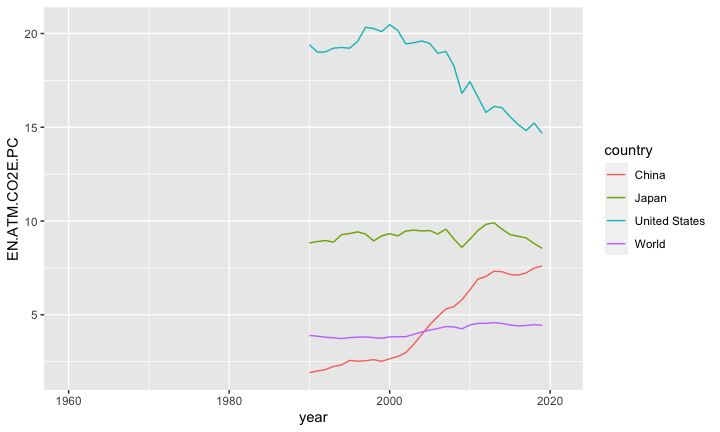
\includegraphics{eda1_files/figure-latex/unnamed-chunk-33-1.pdf}

\hypertarget{comments-on-week-2}{%
\subsection{Comments on Week 2}\label{comments-on-week-2}}

\hypertarget{helpful-resources}{%
\paragraph{Helpful Resources}\label{helpful-resources}}

\begin{itemize}
\item
  Cheat Sheet in RStudio:
  \url{https://www.rstudio.com/resources/cheatsheets/}

  \begin{itemize}
  \tightlist
  \item
    \href{https://raw.githubusercontent.com/rstudio/cheatsheets/main/rstudio-ide.pdf}{RStudio
    IED}
  \item
    \href{https://github.com/rstudio/cheatsheets/raw/main/base-r.pdf}{Base
    R Cheat Sheet}
  \end{itemize}
\item
  `Quick R' by DataCamp: \url{https://www.statmethods.net/management}
\item
  \href{https://cran.rstudio.com}{An Introduction to R}
\end{itemize}

\hypertarget{practicum-1}{%
\paragraph{Practicum}\label{practicum-1}}

\begin{itemize}
\tightlist
\item
  Posit Primers: The Basics: \url{https://posit.cloud/learn/primers/1}

  \begin{itemize}
  \tightlist
  \item
    Complete Visualization Basics and Programming Basics
  \end{itemize}
\end{itemize}

\begin{center}\rule{0.5\linewidth}{0.5pt}\end{center}

\hypertarget{assignments---see-moodle}{%
\paragraph{Assignments - See Moodle}\label{assignments---see-moodle}}

\begin{enumerate}
\def\labelenumi{\arabic{enumi}.}
\tightlist
\item
  Assignment Week 2-1: Introduction Plus Forum\\
\end{enumerate}

\begin{itemize}
\tightlist
\item
  Due: Tuesday, 20 December 2022, 11:59 PM
\end{itemize}

\begin{enumerate}
\def\labelenumi{\arabic{enumi}.}
\setcounter{enumi}{1}
\tightlist
\item
  Assignment Week 2-2: Quiz 1 on R Basics
\end{enumerate}

\begin{itemize}
\tightlist
\item
  Due: Tuesday, 20 December 2022, 11:59 PM
\end{itemize}

\hypertarget{swirl-an-interactive-learning-environment-for-r-and-statistics}{%
\subsection{Swirl: An interactive learning environment for R and
statistics}\label{swirl-an-interactive-learning-environment-for-r-and-statistics}}

\begin{itemize}
\tightlist
\item
  \{\texttt{swirl}\} website: \url{https://swirlstats.com}
\item
  JHU Data Science in coursera uses \texttt{swirl} for exercises.
\end{itemize}

\hypertarget{swirl-courses}{%
\subsubsection{Swirl Courses}\label{swirl-courses}}

\begin{enumerate}
\def\labelenumi{\arabic{enumi}.}
\tightlist
\item
  R Programming: The basics of programming in R
\item
  Regression Models: The basics of regression modeling in R
\item
  Statistical Inference: The basics of statistical inference in R
\item
  Exploratory Data Analysis: The basics of exploring data in R
\end{enumerate}

You can install other \texttt{swirl} courses as well

\begin{itemize}
\tightlist
\item
  \href{http://swirlstats.com/scn/title.html}{Swirl Courses Organized by
  Title}
\item
  \href{http://swirlstats.com/scn/surname.html}{Swirl Courses Organized
  by Author's Name}
\item
  \href{https://github.com/swirldev/swirl_courses\#swirl-courses}{Github:
  swirl courses}

  \begin{itemize}
  \tightlist
  \item
    \texttt{install\_course("Course\ Name\ Here")}
  \end{itemize}
\end{itemize}

\begin{center}\rule{0.5\linewidth}{0.5pt}\end{center}

\hypertarget{install-and-start-swirl-courses}{%
\subsubsection{Install and Start Swirl
Courses}\label{install-and-start-swirl-courses}}

\hypertarget{three-steps-to-start-swirl}{%
\paragraph{Three Steps to Start
Swirl}\label{three-steps-to-start-swirl}}

\begin{verbatim}
install.packages("swirl") # Only the first time.
library(swirl) # Everytime you start swirl
swirl() # Everytime you start or resume swirl
\end{verbatim}

\hypertarget{r-programming-the-basics-of-programming-in-r}{%
\paragraph{R Programming: The basics of programming in
R}\label{r-programming-the-basics-of-programming-in-r}}

\scriptsize

\begin{verbatim}
 1: Basic Building Blocks      2: Workspace and Files     3: Sequences of Numbers    
 4: Vectors                    5: Missing Values          6: Subsetting Vectors      
 7: Matrices and Data Frames   8: Logic                   9: Functions               
10: lapply and sapply         11: vapply and tapply      12: Looking at Data         
13: Simulation                14: Dates and Times        15: Base Graphics          
\end{verbatim}

\hypertarget{recommended-sections-in-order}{%
\paragraph{Recommended Sections in
Order}\label{recommended-sections-in-order}}

1, 3, 4, 5, 6, 7, 12, 15, 14, 8, 9, 10, 11, 13, 2

\begin{itemize}
\tightlist
\item
  Section 2 discusses the directories and file systems of a computer
\item
  Sections 9, 10, 11 are for programming
\end{itemize}

\begin{center}\rule{0.5\linewidth}{0.5pt}\end{center}

\hypertarget{controling-a-swirl-session}{%
\paragraph{\texorpdfstring{Controling a \texttt{swirl}
Session}{Controling a swirl Session}}\label{controling-a-swirl-session}}

\begin{itemize}
\item
  \ldots{} \textless-- That's your cue to press Enter to continue
\item
  You can exit swirl and return to the R prompt (\textgreater) at any
  time by pressing the Esc key.
\item
  If you are already at the prompt, type bye() to exit and save your
  progress. When you exit properly, you'll see a short message letting
  you know you've done so.
\end{itemize}

When you are at the R prompt (\textgreater):

\begin{enumerate}
\def\labelenumi{\arabic{enumi}.}
\tightlist
\item
  Typing skip() allows you to skip the current question.
\item
  Typing play() lets you experiment with R on your own; swirl will
  ignore what you do\ldots{}
\item
  UNTIL you type nxt() which will regain swirl's attention.
\item
  Typing bye() causes swirl to exit. Your progress will be saved.
\item
  Typing main() returns you to swirl's main menu.
\item
  Typing info() displays these options again.
\end{enumerate}

\begin{center}\rule{0.5\linewidth}{0.5pt}\end{center}

\hypertarget{final-remark}{%
\paragraph{Final Remark}\label{final-remark}}

You will encounter the message like `Would you like to receive credit
for completing this course on Coursera.org?' at the end of each course.
This is for \texttt{coursera} courses. Select `NO'.

\hypertarget{more-on-r-script-examples}{%
\subsection{More on R Script:
Examples}\label{more-on-r-script-examples}}

\hypertarget{r-scripts-in-moodle}{%
\subsubsection{R Scripts in Moodle}\label{r-scripts-in-moodle}}

\begin{itemize}
\tightlist
\item
  basics.R
\item
  coronavirus.R
\end{itemize}

\begin{enumerate}
\def\labelenumi{\arabic{enumi}.}
\tightlist
\item
  Copy a script in Moodle: \emph{\{file name\}.R}
\item
  In RStudio (Workspace in RStudio.cloud, Project in RStudio) choose
  File \textgreater{} New File \textgreater{} R Script and paste it.
\item
  Choose File \textgreater{} Save with a name; e.g.~\emph{\{file
  names\}} (.R will be added automatically)
\end{enumerate}

\begin{center}\rule{0.5\linewidth}{0.5pt}\end{center}

\hypertarget{basics.r}{%
\subsubsection{\texorpdfstring{\texttt{basics.R}}{basics.R}}\label{basics.r}}

The script with the outputs.

\begin{Shaded}
\begin{Highlighting}[]
\DocumentationTok{\#\#\#\#\#\#\#\#\#\#\#\#\#\#\#\#\#}
\CommentTok{\#}
\CommentTok{\# basics.R}
\CommentTok{\#}
\DocumentationTok{\#\#\#\#\#\#\#\#\#\#\#\#\#\#\#\#}
\CommentTok{\# \textquotesingle{}Quick R\textquotesingle{} by DataCamp may be a handy reference: }
\CommentTok{\#     https://www.statmethods.net/management/index.html}
\CommentTok{\# Cheat Sheet at RStudio: https://www.rstudio.com/resources/cheatsheets/}
\CommentTok{\# Base R Cheat Sheet: https://github.com/rstudio/cheatsheets/raw/main/base{-}r.pdf}
\CommentTok{\# To execute the line: Control + Enter (Window and Linux), Command + Enter (Mac)}
\DocumentationTok{\#\# try your experiments on the console}

\DocumentationTok{\#\# calculator}

\DecValTok{3} \SpecialCharTok{+} \DecValTok{7}

\DocumentationTok{\#\#\# +, {-}, *, /, \^{} (or **), \%\%, \%/\%}

\DecValTok{3} \SpecialCharTok{+} \DecValTok{10} \SpecialCharTok{/} \DecValTok{2}

\DecValTok{3}\SpecialCharTok{\^{}}\DecValTok{2}

\DecValTok{2}\SpecialCharTok{\^{}}\DecValTok{3}

\DecValTok{2}\SpecialCharTok{*}\DecValTok{2}\SpecialCharTok{*}\DecValTok{2}

\DocumentationTok{\#\#\# assignment: \textless{}{-}, (=, {-}\textgreater{}, assign()) }

\NormalTok{x }\OtherTok{\textless{}{-}} \DecValTok{5}

\NormalTok{x }

\DocumentationTok{\#\#\#\# object\_name \textless{}{-} value, \textquotesingle{}\textless{}{-}\textquotesingle{} shortcut: Alt (option) + \textquotesingle{}{-}\textquotesingle{} (hyphen or minus) }
\DocumentationTok{\#\#\#\# Object names must start with a letter and can only contain letter, numbers, \_ and .}

\NormalTok{this\_is\_a\_long\_name }\OtherTok{\textless{}{-}} \DecValTok{5}\SpecialCharTok{\^{}}\DecValTok{3}

\NormalTok{this\_is\_a\_long\_name}

\NormalTok{char\_name }\OtherTok{\textless{}{-}} \StringTok{"What is your name?"}

\NormalTok{char\_name}

\DocumentationTok{\#\#\#\# Use \textquotesingle{}tab completion\textquotesingle{} and \textquotesingle{}up arrow\textquotesingle{}}

\DocumentationTok{\#\#\# ls(): list of all assignments}

\FunctionTok{ls}\NormalTok{()}
\FunctionTok{ls.str}\NormalTok{()}

\DocumentationTok{\#\#\#\# check Environment in the upper right pane}

\DocumentationTok{\#\#\# (atomic) vectors}

\DecValTok{5}\SpecialCharTok{:}\DecValTok{10}

\NormalTok{a }\OtherTok{\textless{}{-}} \FunctionTok{seq}\NormalTok{(}\DecValTok{5}\NormalTok{,}\DecValTok{10}\NormalTok{)}

\NormalTok{a}

\NormalTok{b }\OtherTok{\textless{}{-}} \DecValTok{5}\SpecialCharTok{:}\DecValTok{10}

\FunctionTok{identical}\NormalTok{(a,b)}

\FunctionTok{seq}\NormalTok{(}\DecValTok{5}\NormalTok{,}\DecValTok{10}\NormalTok{,}\DecValTok{2}\NormalTok{) }\CommentTok{\# same as seq(from = 5, to = 10, by = 2)}

\NormalTok{c1 }\OtherTok{\textless{}{-}} \FunctionTok{seq}\NormalTok{(}\DecValTok{0}\NormalTok{,}\DecValTok{100}\NormalTok{, }\AttributeTok{by =} \DecValTok{10}\NormalTok{)}

\NormalTok{c2 }\OtherTok{\textless{}{-}} \FunctionTok{seq}\NormalTok{(}\DecValTok{0}\NormalTok{,}\DecValTok{100}\NormalTok{, }\AttributeTok{length.out =} \DecValTok{10}\NormalTok{)}

\NormalTok{c1}

\NormalTok{c2}

\FunctionTok{length}\NormalTok{(c1)}

\DocumentationTok{\#\#\#\# ? seq   ? length   ? identical}

\NormalTok{(die }\OtherTok{\textless{}{-}} \DecValTok{1}\SpecialCharTok{:}\DecValTok{6}\NormalTok{)}

\NormalTok{zero\_one }\OtherTok{\textless{}{-}} \FunctionTok{c}\NormalTok{(}\DecValTok{0}\NormalTok{,}\DecValTok{1}\NormalTok{) }\CommentTok{\# same as 0:1}

\NormalTok{die }\SpecialCharTok{+}\NormalTok{ zero\_one }\CommentTok{\# c(1,2,3,4,5,6) + c(0,1). re{-}use}

\NormalTok{d1 }\OtherTok{\textless{}{-}} \FunctionTok{rep}\NormalTok{(}\DecValTok{1}\SpecialCharTok{:}\DecValTok{3}\NormalTok{,}\DecValTok{2}\NormalTok{) }\CommentTok{\# repeat}


\NormalTok{d1}

\NormalTok{die }\SpecialCharTok{==}\NormalTok{ d1}

\NormalTok{d2 }\OtherTok{\textless{}{-}} \FunctionTok{as.character}\NormalTok{(die }\SpecialCharTok{==}\NormalTok{ d1)}

\NormalTok{d2}

\NormalTok{d3 }\OtherTok{\textless{}{-}} \FunctionTok{as.numeric}\NormalTok{(die }\SpecialCharTok{==}\NormalTok{ d1)}

\NormalTok{d3}

\DocumentationTok{\#\#\# class() for class and typeof() for mode}
\DocumentationTok{\#\#\# class of vectors: numeric, charcters, logical}
\DocumentationTok{\#\#\# types of vectors: doubles, integers, characters, logicals (complex and raw)}

\FunctionTok{typeof}\NormalTok{(d1); }\FunctionTok{class}\NormalTok{(d1)}

\FunctionTok{typeof}\NormalTok{(d2); }\FunctionTok{class}\NormalTok{(d2)}

\FunctionTok{typeof}\NormalTok{(d3); }\FunctionTok{class}\NormalTok{(d3)}

\FunctionTok{sqrt}\NormalTok{(}\DecValTok{2}\NormalTok{)}

\FunctionTok{sqrt}\NormalTok{(}\DecValTok{2}\NormalTok{)}\SpecialCharTok{\^{}}\DecValTok{2}

\FunctionTok{sqrt}\NormalTok{(}\DecValTok{2}\NormalTok{)}\SpecialCharTok{\^{}}\DecValTok{2} \SpecialCharTok{{-}} \DecValTok{2}

\FunctionTok{typeof}\NormalTok{(}\FunctionTok{sqrt}\NormalTok{(}\DecValTok{2}\NormalTok{))}

\FunctionTok{typeof}\NormalTok{(}\DecValTok{2}\NormalTok{)}

\FunctionTok{typeof}\NormalTok{(2L)}

\DecValTok{5} \SpecialCharTok{==} \FunctionTok{c}\NormalTok{(}\DecValTok{5}\NormalTok{)}

\FunctionTok{length}\NormalTok{(}\DecValTok{5}\NormalTok{)}

\DocumentationTok{\#\#\# Subsetting}

\NormalTok{(A\_Z }\OtherTok{\textless{}{-}}\NormalTok{ LETTERS)}

\NormalTok{A\_F }\OtherTok{\textless{}{-}}\NormalTok{ A\_Z[}\DecValTok{1}\SpecialCharTok{:}\DecValTok{6}\NormalTok{]}

\NormalTok{A\_F}

\NormalTok{A\_F[}\DecValTok{3}\NormalTok{]}

\NormalTok{A\_F[}\FunctionTok{c}\NormalTok{(}\DecValTok{3}\NormalTok{,}\DecValTok{5}\NormalTok{)]}

\NormalTok{large }\OtherTok{\textless{}{-}}\NormalTok{ die }\SpecialCharTok{\textgreater{}} \DecValTok{3}

\NormalTok{large}

\NormalTok{even }\OtherTok{\textless{}{-}}\NormalTok{ die }\SpecialCharTok{\%in\%} \FunctionTok{c}\NormalTok{(}\DecValTok{2}\NormalTok{,}\DecValTok{4}\NormalTok{,}\DecValTok{6}\NormalTok{)}

\NormalTok{even}

\NormalTok{A\_F[large]}

\NormalTok{A\_F[even]}

\NormalTok{A\_F[die }\SpecialCharTok{\textless{}} \DecValTok{4}\NormalTok{]}

\DocumentationTok{\#\#\# Compare df with df1 \textless{}{-} data.frame(number = die, alphabet = A\_F)}
\NormalTok{df }\OtherTok{\textless{}{-}} \FunctionTok{data.frame}\NormalTok{(}\AttributeTok{number =}\NormalTok{ die, }\AttributeTok{alphabet =}\NormalTok{ A\_F, }\AttributeTok{stringsAsFactors =} \ConstantTok{FALSE}\NormalTok{)}

\NormalTok{df}

\NormalTok{df}\SpecialCharTok{$}\NormalTok{number}

\NormalTok{df}\SpecialCharTok{$}\NormalTok{alphabet}

\NormalTok{df[}\DecValTok{3}\NormalTok{,}\DecValTok{2}\NormalTok{]}

\NormalTok{df[}\DecValTok{4}\NormalTok{,}\DecValTok{1}\NormalTok{]}

\NormalTok{df[}\DecValTok{1}\NormalTok{]}

\FunctionTok{class}\NormalTok{(df[}\DecValTok{1}\NormalTok{])}

\FunctionTok{class}\NormalTok{(df[[}\DecValTok{1}\NormalTok{]])}

\FunctionTok{identical}\NormalTok{(df[[}\DecValTok{1}\NormalTok{]], die)}

\FunctionTok{identical}\NormalTok{(df[}\DecValTok{1}\NormalTok{],die)}

\DocumentationTok{\#\#\#\#\#\#\#\#\#\#\#\#\#\#\#\#\#\#\#\#}
\CommentTok{\# The First Example}
\DocumentationTok{\#\#\#\#\#\#\#\#\#\#\#\#\#\#\#\#\#\#\#\#}

\FunctionTok{plot}\NormalTok{(cars)}

\CommentTok{\# Help}

\NormalTok{? cars}

\CommentTok{\# cars is in the \textquotesingle{}datasets\textquotesingle{} package}

\FunctionTok{data}\NormalTok{()}

\CommentTok{\# help(cars) does the same as ? cars}
\CommentTok{\# You can use Help tab in the right bottom pane}

\FunctionTok{help}\NormalTok{(plot)}
\NormalTok{? par}

\FunctionTok{head}\NormalTok{(cars)}

\FunctionTok{str}\NormalTok{(cars)}

\FunctionTok{summary}\NormalTok{(cars)}

\NormalTok{x }\OtherTok{\textless{}{-}}\NormalTok{ cars}\SpecialCharTok{$}\NormalTok{speed}
\NormalTok{y }\OtherTok{\textless{}{-}}\NormalTok{ cars}\SpecialCharTok{$}\NormalTok{dist}

\FunctionTok{min}\NormalTok{(x)}
\FunctionTok{mean}\NormalTok{(x)}
\FunctionTok{quantile}\NormalTok{(x)}

\FunctionTok{plot}\NormalTok{(cars)}

\FunctionTok{abline}\NormalTok{(}\FunctionTok{lm}\NormalTok{(cars}\SpecialCharTok{$}\NormalTok{dist }\SpecialCharTok{\textasciitilde{}}\NormalTok{ cars}\SpecialCharTok{$}\NormalTok{speed))}

\FunctionTok{summary}\NormalTok{(}\FunctionTok{lm}\NormalTok{(cars}\SpecialCharTok{$}\NormalTok{dist }\SpecialCharTok{\textasciitilde{}}\NormalTok{ cars}\SpecialCharTok{$}\NormalTok{speed))}

\FunctionTok{boxplot}\NormalTok{(cars)}

\FunctionTok{hist}\NormalTok{(cars}\SpecialCharTok{$}\NormalTok{speed)}
\FunctionTok{hist}\NormalTok{(cars}\SpecialCharTok{$}\NormalTok{dist)}
\FunctionTok{hist}\NormalTok{(cars}\SpecialCharTok{$}\NormalTok{dist, }\AttributeTok{breaks =} \FunctionTok{seq}\NormalTok{(}\DecValTok{0}\NormalTok{,}\DecValTok{120}\NormalTok{, }\DecValTok{10}\NormalTok{))}
\end{Highlighting}
\end{Shaded}

\begin{center}\rule{0.5\linewidth}{0.5pt}\end{center}

\hypertarget{coronavirus.r}{%
\subsubsection{coronavirus.R}\label{coronavirus.r}}

The script and its outputs. \textbf{coronavirus.csv} is very large

\begin{Shaded}
\begin{Highlighting}[]
\CommentTok{\# https://coronavirus.jhu.edu/map.html}
\CommentTok{\# JHU Covid{-}19 global time series data}
\CommentTok{\# See R pakage coronavirus at: https://github.com/RamiKrispin/coronavirus}
\CommentTok{\# Data taken from: https://github.com/RamiKrispin/coronavirus/tree/master/csv}
\CommentTok{\# Last Updated}
\FunctionTok{Sys.Date}\NormalTok{()}

\DocumentationTok{\#\# Download and read csv (comma separated value) file}
\NormalTok{coronavirus }\OtherTok{\textless{}{-}} \FunctionTok{read.csv}\NormalTok{(}\StringTok{"https://github.com/RamiKrispin/coronavirus/raw/master/csv/coronavirus.csv"}\NormalTok{)}
\CommentTok{\# write.csv(coronavirus, "data/coronavirus.csv")}

\DocumentationTok{\#\# Summaries and structures of the data}
\FunctionTok{head}\NormalTok{(coronavirus)}
\FunctionTok{str}\NormalTok{(coronavirus)}
\NormalTok{coronavirus}\SpecialCharTok{$}\NormalTok{date }\OtherTok{\textless{}{-}} \FunctionTok{as.Date}\NormalTok{(coronavirus}\SpecialCharTok{$}\NormalTok{date)}
\FunctionTok{str}\NormalTok{(coronavirus)}

\FunctionTok{range}\NormalTok{(coronavirus}\SpecialCharTok{$}\NormalTok{date)}
\FunctionTok{unique}\NormalTok{(coronavirus}\SpecialCharTok{$}\NormalTok{country)}
\FunctionTok{unique}\NormalTok{(coronavirus}\SpecialCharTok{$}\NormalTok{type)}

\DocumentationTok{\#\# Set Country}
\NormalTok{COUNTRY }\OtherTok{\textless{}{-}} \StringTok{"Japan"}
\NormalTok{df0 }\OtherTok{\textless{}{-}}\NormalTok{ coronavirus[coronavirus}\SpecialCharTok{$}\NormalTok{country }\SpecialCharTok{==}\NormalTok{ COUNTRY,]}
\FunctionTok{head}\NormalTok{(df0)}
\FunctionTok{tail}\NormalTok{(df0)}
\NormalTok{(pop }\OtherTok{\textless{}{-}}\NormalTok{ df0}\SpecialCharTok{$}\NormalTok{population[}\DecValTok{1}\NormalTok{])}
\NormalTok{df }\OtherTok{\textless{}{-}}\NormalTok{ df0[}\FunctionTok{c}\NormalTok{(}\DecValTok{1}\NormalTok{,}\DecValTok{6}\NormalTok{,}\DecValTok{7}\NormalTok{,}\DecValTok{13}\NormalTok{)]}
\FunctionTok{str}\NormalTok{(df)}
\FunctionTok{head}\NormalTok{(df)}
\DocumentationTok{\#\#\# alternatively,}
\FunctionTok{head}\NormalTok{(df0[}\FunctionTok{c}\NormalTok{(}\StringTok{"date"}\NormalTok{, }\StringTok{"type"}\NormalTok{, }\StringTok{"cases"}\NormalTok{, }\StringTok{"population"}\NormalTok{)])}
\DocumentationTok{\#\#\#}

\DocumentationTok{\#\# Set types}
\NormalTok{df\_confirmed }\OtherTok{\textless{}{-}}\NormalTok{ df[df}\SpecialCharTok{$}\NormalTok{type }\SpecialCharTok{==} \StringTok{"confirmed"}\NormalTok{,]}
\NormalTok{df\_death }\OtherTok{\textless{}{-}}\NormalTok{ df[df}\SpecialCharTok{$}\NormalTok{type }\SpecialCharTok{==} \StringTok{"death"}\NormalTok{,]}
\NormalTok{df\_recovery }\OtherTok{\textless{}{-}}\NormalTok{ df[df}\SpecialCharTok{$}\NormalTok{data\_type }\SpecialCharTok{==} \StringTok{"recovery"}\NormalTok{,]}
\FunctionTok{head}\NormalTok{(df\_confirmed)}
\FunctionTok{head}\NormalTok{(df\_death)}
\FunctionTok{head}\NormalTok{(df\_recovery)}

\DocumentationTok{\#\# Histogram}
\FunctionTok{plot}\NormalTok{(df\_confirmed}\SpecialCharTok{$}\NormalTok{date, df\_confirmed}\SpecialCharTok{$}\NormalTok{cases, }\AttributeTok{type =} \StringTok{"h"}\NormalTok{)}
\FunctionTok{plot}\NormalTok{(df\_death}\SpecialCharTok{$}\NormalTok{date, df\_death}\SpecialCharTok{$}\NormalTok{cases, }\AttributeTok{type =} \StringTok{"h"}\NormalTok{)}
\CommentTok{\# plot(df\_recovered$date, df\_recovered$cases, type = "h") \# no data for recovery}

\DocumentationTok{\#\# Scatter plot and correlation}
\FunctionTok{plot}\NormalTok{(df\_confirmed}\SpecialCharTok{$}\NormalTok{cases, df\_death}\SpecialCharTok{$}\NormalTok{cases, }\AttributeTok{type =} \StringTok{"p"}\NormalTok{)}
\FunctionTok{cor}\NormalTok{(df\_confirmed}\SpecialCharTok{$}\NormalTok{cases, df\_death}\SpecialCharTok{$}\NormalTok{cases)}


\DocumentationTok{\#\# In addition set a period}
\NormalTok{start\_date }\OtherTok{\textless{}{-}} \FunctionTok{as.Date}\NormalTok{(}\StringTok{"2021{-}07{-}01"}\NormalTok{)}
\NormalTok{end\_date }\OtherTok{\textless{}{-}} \FunctionTok{Sys.Date}\NormalTok{() }
\NormalTok{df\_date }\OtherTok{\textless{}{-}}\NormalTok{ df[df}\SpecialCharTok{$}\NormalTok{date }\SpecialCharTok{\textgreater{}=}\NormalTok{start\_date }\SpecialCharTok{\&}\NormalTok{ df}\SpecialCharTok{$}\NormalTok{date }\SpecialCharTok{\textless{}=}\NormalTok{ end\_date,]}
\DocumentationTok{\#\#}

\DocumentationTok{\#\# Set types}
\NormalTok{df\_date\_confirmed }\OtherTok{\textless{}{-}}\NormalTok{ df\_date[df\_date}\SpecialCharTok{$}\NormalTok{type }\SpecialCharTok{==} \StringTok{"confirmed"}\NormalTok{,]}
\NormalTok{df\_date\_death }\OtherTok{\textless{}{-}}\NormalTok{ df\_date[df\_date}\SpecialCharTok{$}\NormalTok{type }\SpecialCharTok{==} \StringTok{"death"}\NormalTok{,]}
\NormalTok{df\_date\_recovery }\OtherTok{\textless{}{-}}\NormalTok{ df\_date[df\_date}\SpecialCharTok{$}\NormalTok{data\_type }\SpecialCharTok{==} \StringTok{"recovery"}\NormalTok{,]}
\FunctionTok{head}\NormalTok{(df\_date\_confirmed)}
\FunctionTok{head}\NormalTok{(df\_date\_death)}
\FunctionTok{head}\NormalTok{(df\_date\_recovery)}

\DocumentationTok{\#\# Histogram}
\FunctionTok{plot}\NormalTok{(df\_date\_confirmed}\SpecialCharTok{$}\NormalTok{date, df\_date\_confirmed}\SpecialCharTok{$}\NormalTok{cases, }\AttributeTok{type =} \StringTok{"h"}\NormalTok{)}
\FunctionTok{plot}\NormalTok{(df\_date\_death}\SpecialCharTok{$}\NormalTok{date, df\_date\_death}\SpecialCharTok{$}\NormalTok{cases, }\AttributeTok{type =} \StringTok{"h"}\NormalTok{)}
\CommentTok{\# plot(df\_date\_recovered$date, df\_date\_recovered$cases, type = "h") \# no data for recovery}

\FunctionTok{plot}\NormalTok{(df\_date\_confirmed}\SpecialCharTok{$}\NormalTok{cases, df\_date\_death}\SpecialCharTok{$}\NormalTok{cases, }\AttributeTok{type =} \StringTok{"p"}\NormalTok{)}
\FunctionTok{cor}\NormalTok{(df\_date\_confirmed}\SpecialCharTok{$}\NormalTok{cases, df\_date\_death}\SpecialCharTok{$}\NormalTok{cases)}

\DocumentationTok{\#\#\# Q0. Change the values of the location and the period and see the outcomes.}
\DocumentationTok{\#\#\# Q1. What is the correlation between df\_confirmed$cases and df\_death$cases?}
\DocumentationTok{\#\#\# Q2. Do we have a larger correlation value if we shift the dates to implement the time{-}lag?}
\DocumentationTok{\#\#\# Q3. Do you have any other questions to explore?}

\DocumentationTok{\#\#\#\# Extra}
\FunctionTok{plot}\NormalTok{(df\_confirmed}\SpecialCharTok{$}\NormalTok{date, df\_confirmed}\SpecialCharTok{$}\NormalTok{cases, }\AttributeTok{type =} \StringTok{"h"}\NormalTok{, }
     \AttributeTok{main =} \FunctionTok{paste}\NormalTok{(}\StringTok{"Comfirmed Cases in"}\NormalTok{,COUNTRY), }
     \AttributeTok{xlab =} \StringTok{"Date"}\NormalTok{, }\AttributeTok{ylab =} \StringTok{"Number of Cases"}\NormalTok{)}
\end{Highlighting}
\end{Shaded}

:::

\hypertarget{gapminder-package}{%
\subsection{\texorpdfstring{\texttt{gapminder}
Package}{gapminder Package}}\label{gapminder-package}}

\hypertarget{hans-rosling-1948-2017}{%
\subsubsection{Hans Rosling (1948 --
2017)}\label{hans-rosling-1948-2017}}

\begin{quote}
Hans Rosling was a Swedish physician, academic, and public speaker. He
was a professor of international health at Karolinska Institute{[}4{]}
and was the co-founder and chairman of the Gapminder Foundation, which
developed the Trendalyzer software system.
(\href{https://en.wikipedia.org/wiki/Hans_Rosling}{wikipedia})
\end{quote}

\begin{itemize}
\tightlist
\item
  Books:

  \begin{itemize}
  \tightlist
  \item
    Factfulness: Ten Reasons We're Wrong About The World - And Why
    Things Are Better Than You Think, 2018
  \item
    How I Learned to Understand the World: A Memoir, 2020
  \end{itemize}
\item
  Gapminder: \url{https://www.gapminder.org}

  \begin{itemize}
  \tightlist
  \item
    \href{https://upgrader.gapminder.org}{You are probably wrong about:
    Upgrade Your World View}
  \item
    \href{https://www.gapminder.org/tools/\#$state$time$value=2020;;\&chart-type=bubbles}{Bubble
    Chart}: Income vs Life Expectancy over time, 1800 - 2020

    \begin{itemize}
    \tightlist
    \item
      How many variables?
    \end{itemize}
  \end{itemize}
\item
  Videos:
  \href{http://www.edtech.events/the-best-stats-youve-ever-seen-hans-rosling/}{The
  best stats you've ever seen, Hans Rosling}
\end{itemize}

\begin{center}\rule{0.5\linewidth}{0.5pt}\end{center}

\hypertarget{factfulness-is-from-the-book}{%
\subsubsection{\texorpdfstring{Factfulness is \ldots{} \hfill \emph{From
the
book}}{Factfulness is \ldots{} From the book}}\label{factfulness-is-from-the-book}}

recognizing when a decision feels urgent and remembering that it rarely
is.

To control the urgency instinct, take small steps.

\begin{itemize}
\tightlist
\item
  Take a breath. When your urgency instinct is triggered, your other
  instincts kick in and your analysis shuts down. Ask for more time and
  more information. It's rarely now or never and it's rarely either/or.
\item
  Insist on the data. If something is urgent and important, it should be
  measured. Beware of data that is relevant but inaccurate, or accurate
  but irrelevant. Only relevant and accurate data is useful.
\item
  Beware of fortune-tellers. Any prediction about the future is
  uncertain. Be wary of predictions that fail to acknowledge that.
  Insist on a full range of scenarios, never just the best or worst
  case. Ask how often such predictions have been right before.
\item
  Be wary of drastic action. Ask what the side effects will be. Ask how
  the idea has been tested. Step-by-step practical improvements, and
  evaluation of their impact, are less dramatic but usually more
  effective.
\end{itemize}

\begin{center}\rule{0.5\linewidth}{0.5pt}\end{center}

\begin{Shaded}
\begin{Highlighting}[]
\CommentTok{\# install.packages("gapminder")}
\FunctionTok{library}\NormalTok{(gapminder)}
\end{Highlighting}
\end{Shaded}

\begin{Shaded}
\begin{Highlighting}[]
\NormalTok{df }\OtherTok{\textless{}{-}}\NormalTok{ gapminder}
\NormalTok{df}
\end{Highlighting}
\end{Shaded}

\begin{verbatim}
## # A tibble: 1,704 x 6
##    country     continent  year lifeExp      pop gdpPercap
##    <fct>       <fct>     <int>   <dbl>    <int>     <dbl>
##  1 Afghanistan Asia       1952    28.8  8425333      779.
##  2 Afghanistan Asia       1957    30.3  9240934      821.
##  3 Afghanistan Asia       1962    32.0 10267083      853.
##  4 Afghanistan Asia       1967    34.0 11537966      836.
##  5 Afghanistan Asia       1972    36.1 13079460      740.
##  6 Afghanistan Asia       1977    38.4 14880372      786.
##  7 Afghanistan Asia       1982    39.9 12881816      978.
##  8 Afghanistan Asia       1987    40.8 13867957      852.
##  9 Afghanistan Asia       1992    41.7 16317921      649.
## 10 Afghanistan Asia       1997    41.8 22227415      635.
## # ... with 1,694 more rows
\end{verbatim}

\begin{center}\rule{0.5\linewidth}{0.5pt}\end{center}

\begin{Shaded}
\begin{Highlighting}[]
\FunctionTok{glimpse}\NormalTok{(df)}
\end{Highlighting}
\end{Shaded}

\begin{verbatim}
## Rows: 1,704
## Columns: 6
## $ country   <fct> "Afghanistan", "Afghanistan", "Afghanistan", "Afghanistan", ~
## $ continent <fct> Asia, Asia, Asia, Asia, Asia, Asia, Asia, Asia, Asia, Asia, ~
## $ year      <int> 1952, 1957, 1962, 1967, 1972, 1977, 1982, 1987, 1992, 1997, ~
## $ lifeExp   <dbl> 28.801, 30.332, 31.997, 34.020, 36.088, 38.438, 39.854, 40.8~
## $ pop       <int> 8425333, 9240934, 10267083, 11537966, 13079460, 14880372, 12~
## $ gdpPercap <dbl> 779.4453, 820.8530, 853.1007, 836.1971, 739.9811, 786.1134, ~
\end{verbatim}

\begin{center}\rule{0.5\linewidth}{0.5pt}\end{center}

\begin{Shaded}
\begin{Highlighting}[]
\FunctionTok{summary}\NormalTok{(df)}
\end{Highlighting}
\end{Shaded}

\begin{verbatim}
##         country        continent        year         lifeExp     
##  Afghanistan:  12   Africa  :624   Min.   :1952   Min.   :23.60  
##  Albania    :  12   Americas:300   1st Qu.:1966   1st Qu.:48.20  
##  Algeria    :  12   Asia    :396   Median :1980   Median :60.71  
##  Angola     :  12   Europe  :360   Mean   :1980   Mean   :59.47  
##  Argentina  :  12   Oceania : 24   3rd Qu.:1993   3rd Qu.:70.85  
##  Australia  :  12                  Max.   :2007   Max.   :82.60  
##  (Other)    :1632                                                
##       pop              gdpPercap       
##  Min.   :6.001e+04   Min.   :   241.2  
##  1st Qu.:2.794e+06   1st Qu.:  1202.1  
##  Median :7.024e+06   Median :  3531.8  
##  Mean   :2.960e+07   Mean   :  7215.3  
##  3rd Qu.:1.959e+07   3rd Qu.:  9325.5  
##  Max.   :1.319e+09   Max.   :113523.1  
## 
\end{verbatim}

\begin{center}\rule{0.5\linewidth}{0.5pt}\end{center}

\hypertarget{questions}{%
\subsubsection{Questions}\label{questions}}

\begin{itemize}
\tightlist
\item
  List questions based on this data.
\item
  What do you want to see?
\item
  What kind of chart do you want to construct?
\end{itemize}

\end{document}
